%\documentclass[12pt]{article}
%\usepackage[utf8]{inputenc}
%\usepackage[left=2cm,right=2cm,top=2cm,bottom=2cm]{geometry}
%\usepackage{pdfpages, subcaption, url}
%
%\begin{document}
%
%\thispagestyle{empty}
\begin{scshape}
\begin{center}
	{\Large{Universidad Autónoma de Nuevo León}} \\[5mm]
	{\large{Facultad de Ingeniería Mecánica y Eléctrica}} \\[5mm]
	{\large{Posgrado en Ingeniería de Sistemas}} \\[5 mm]
	{\large{Doctorado}}
	\vskip16mm
	\begin{figure}[h!]
		\centering
		\begin{subfigure}{0.3\linewidth}
			\includegraphics[width=\linewidth]{images/uanl}
		\end{subfigure}
		\hspace{15 mm}
		\begin{subfigure}{0.2\linewidth}
			\includegraphics[width=\linewidth]{images/fime}
		\end{subfigure}
	\end{figure}
	\vskip16mm
	\begin{tabular}{p{11cm}}
		\centering
		{\large Portafolio de Evidencias}
	\end{tabular}
	\vskip7mm
	{de}\\[7mm]
	{\large Gabriela Sánchez Yepez}\\[3mm]
	{1935064}\\[7 mm]
	{para el curso de Modelos Probabilistas Aplicados,}\\[3mm]
	{con la profesora Dra. Satu Elisa Schaeffer.}\\[3mm]
	Semestre Agosto 2020 - Enero 2021. \\ [5 mm]
	\url{https://github.com/Saphira3000/MPA}
	\vfill
\end{center}
\end{scshape}
%
%%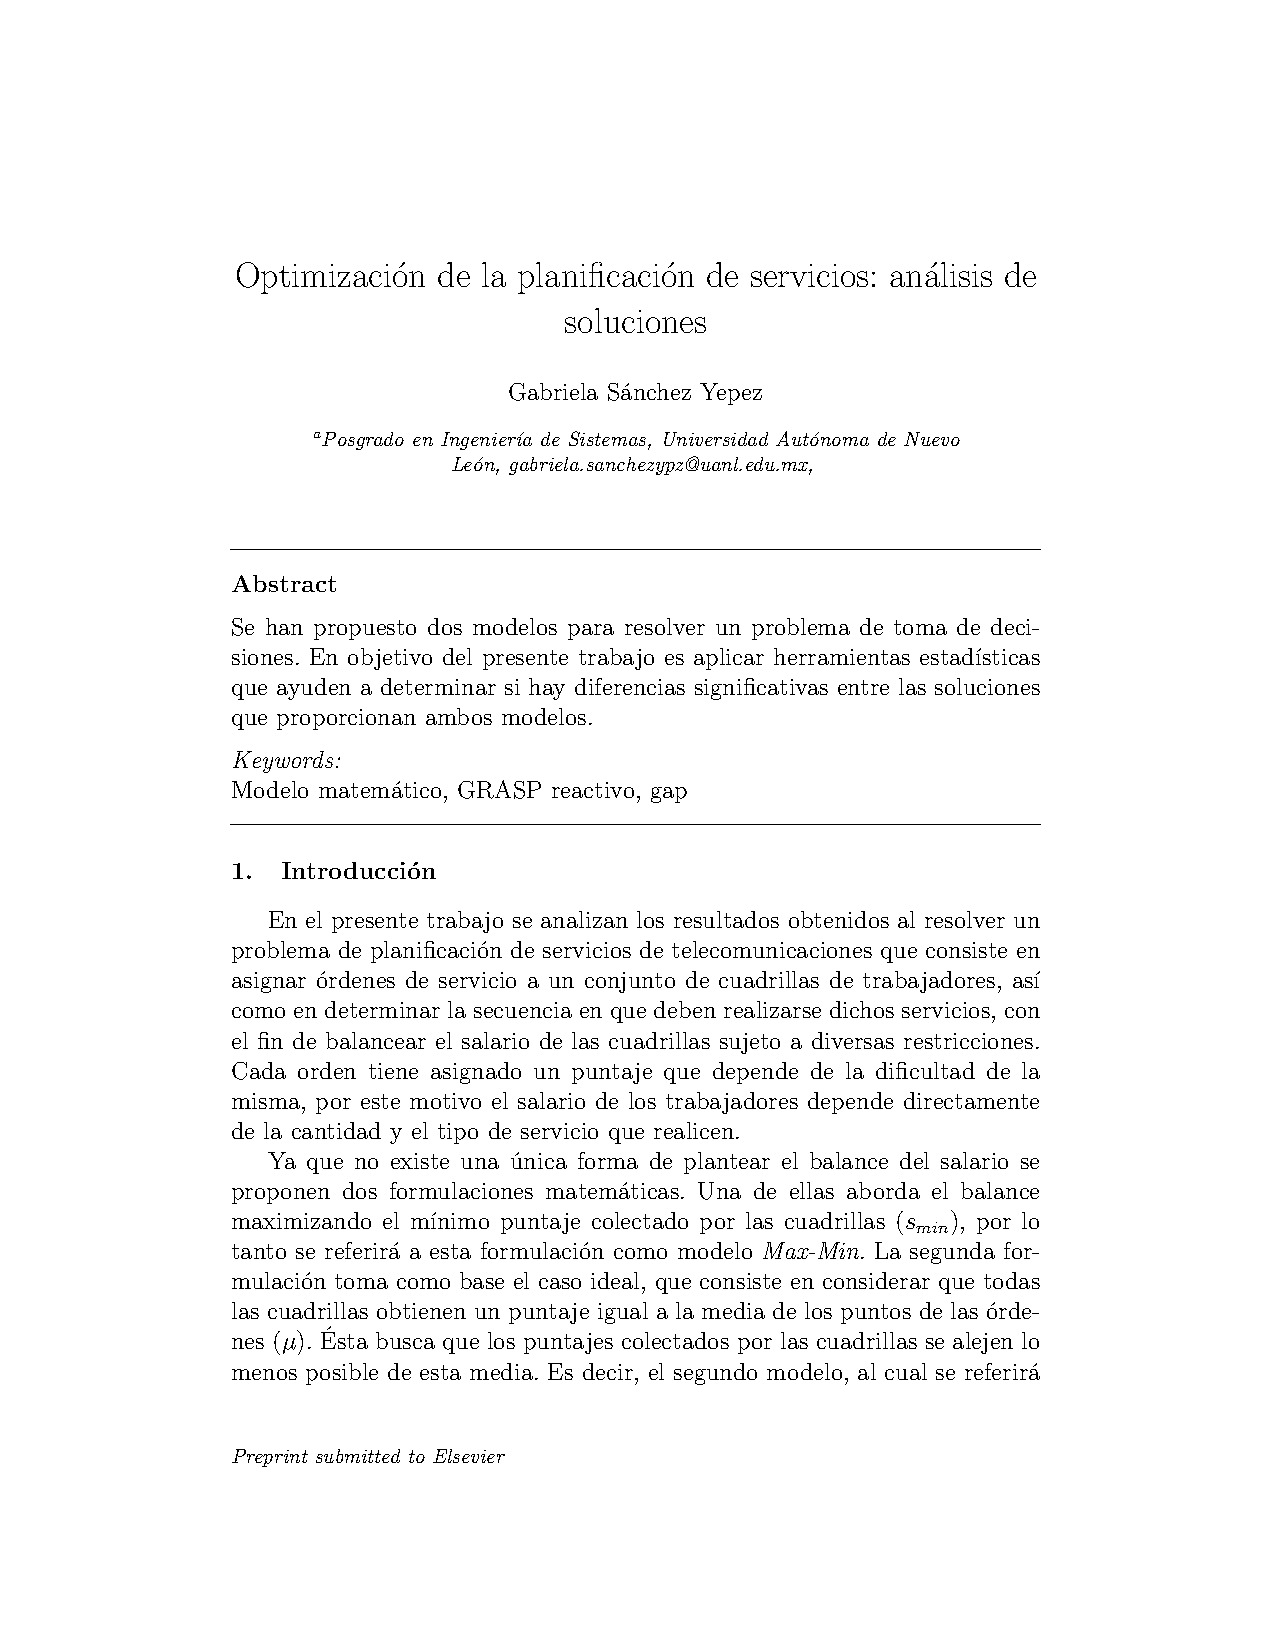
\includepdf[pages=1-2]{proyecto.pdf}
%
%
%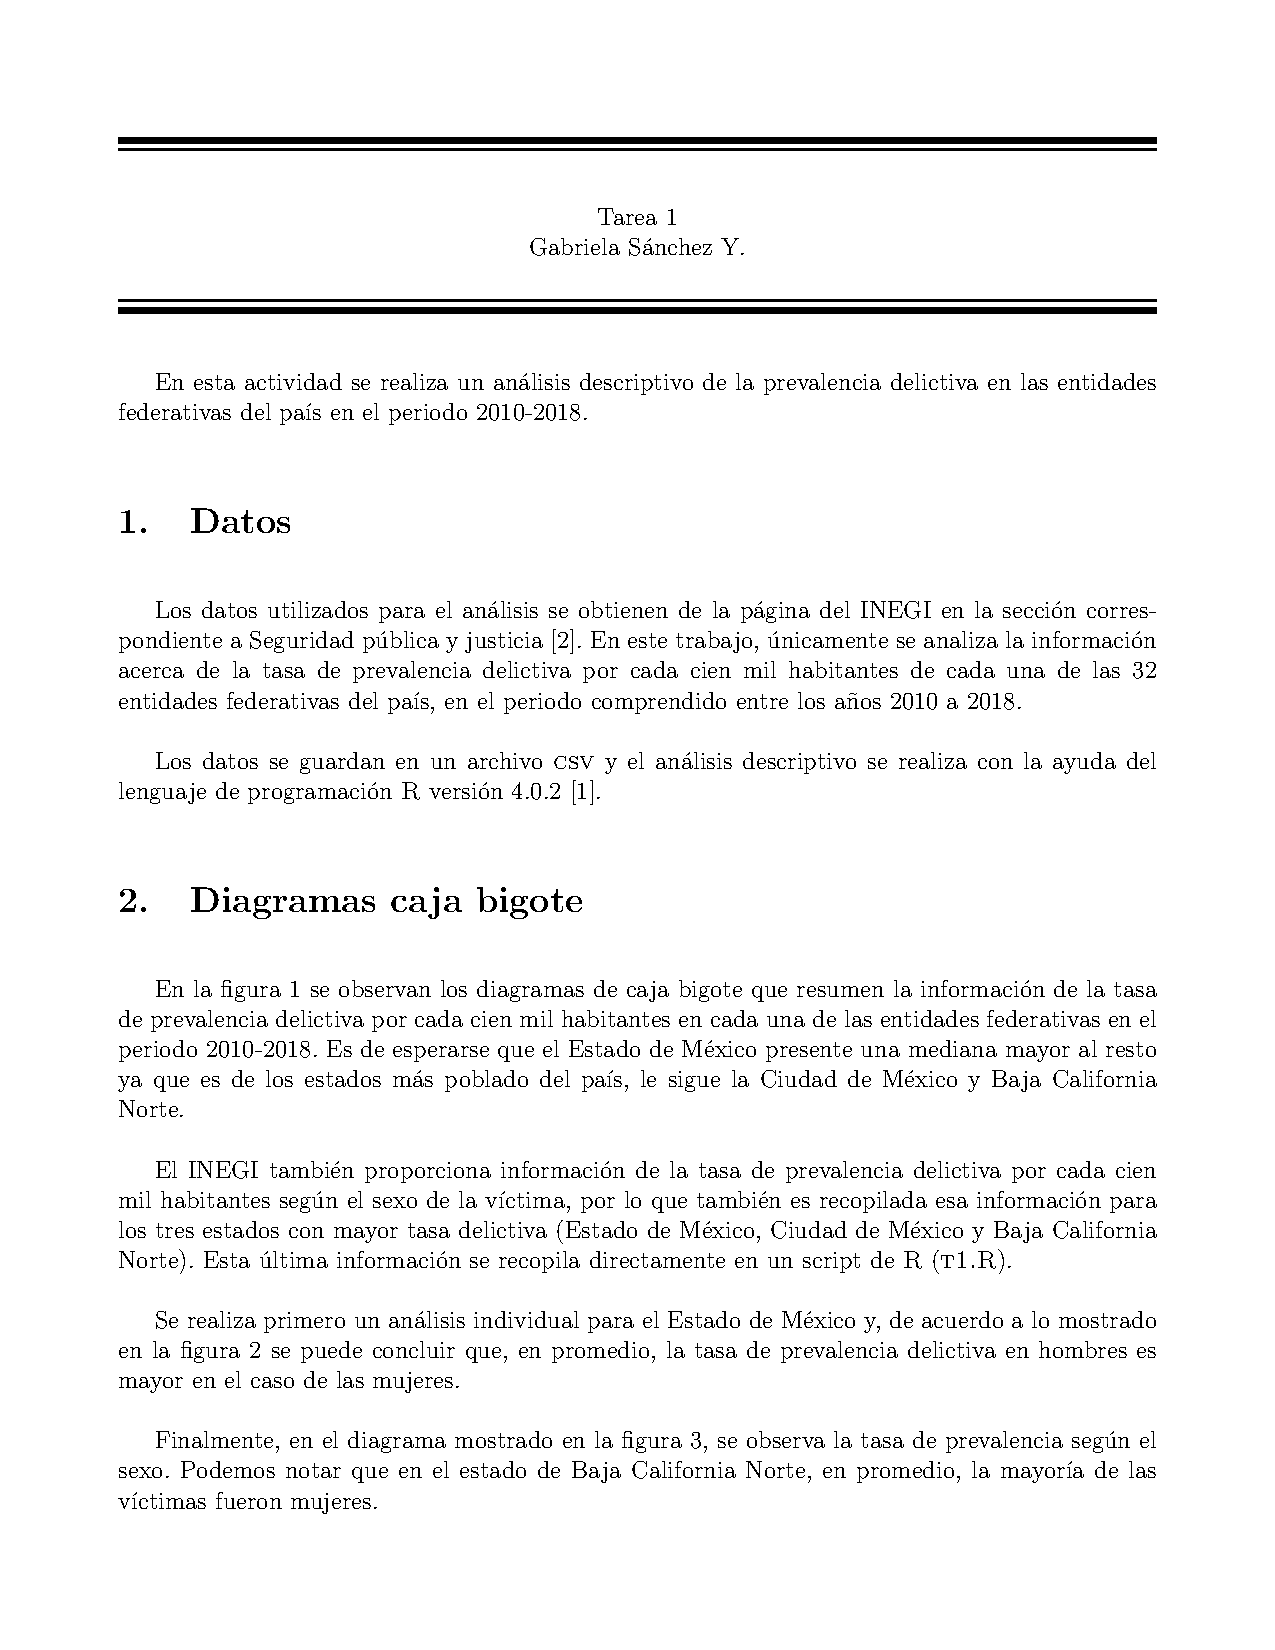
\includepdf[pages=-,pagecommand={\section{Tarea 1}\label{t1}},linktodoc=true]{t1.pdf}
%%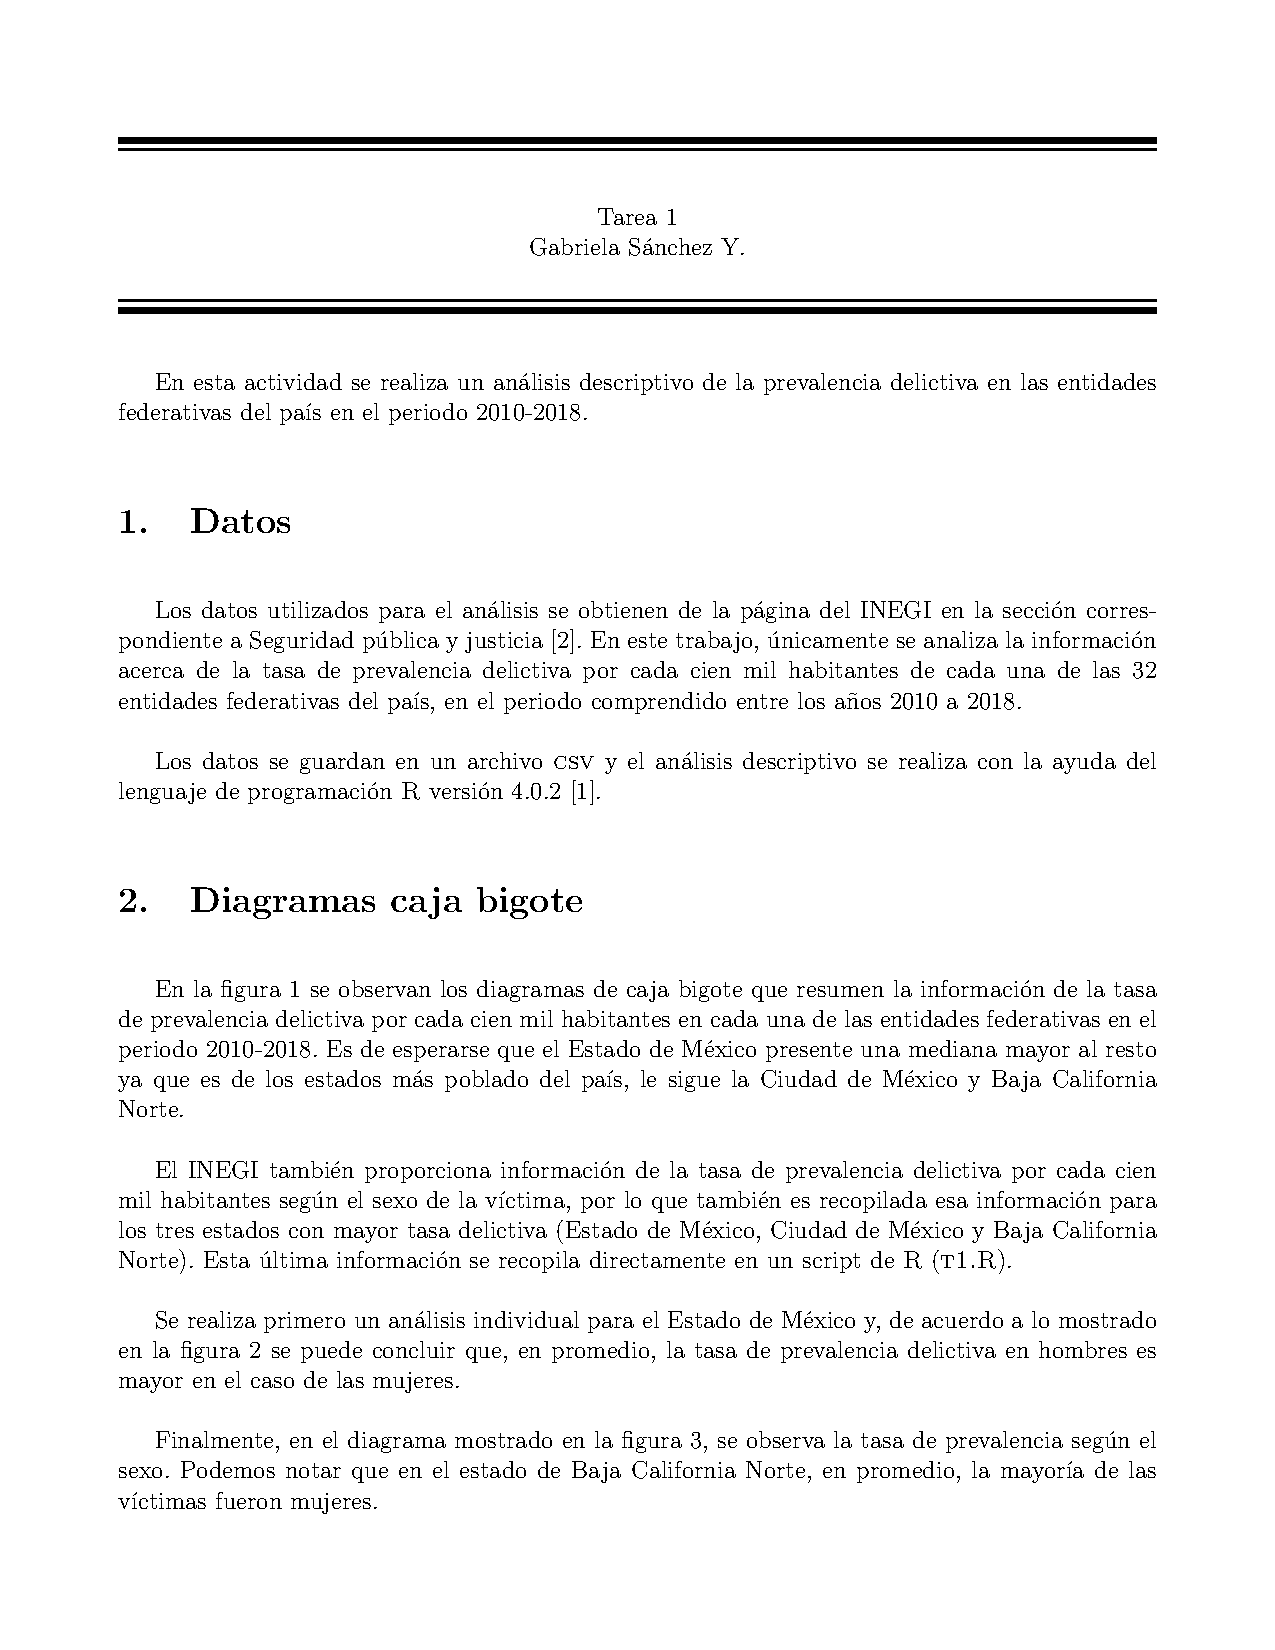
\includepdf[pages=1-3]{t1.pdf}
%%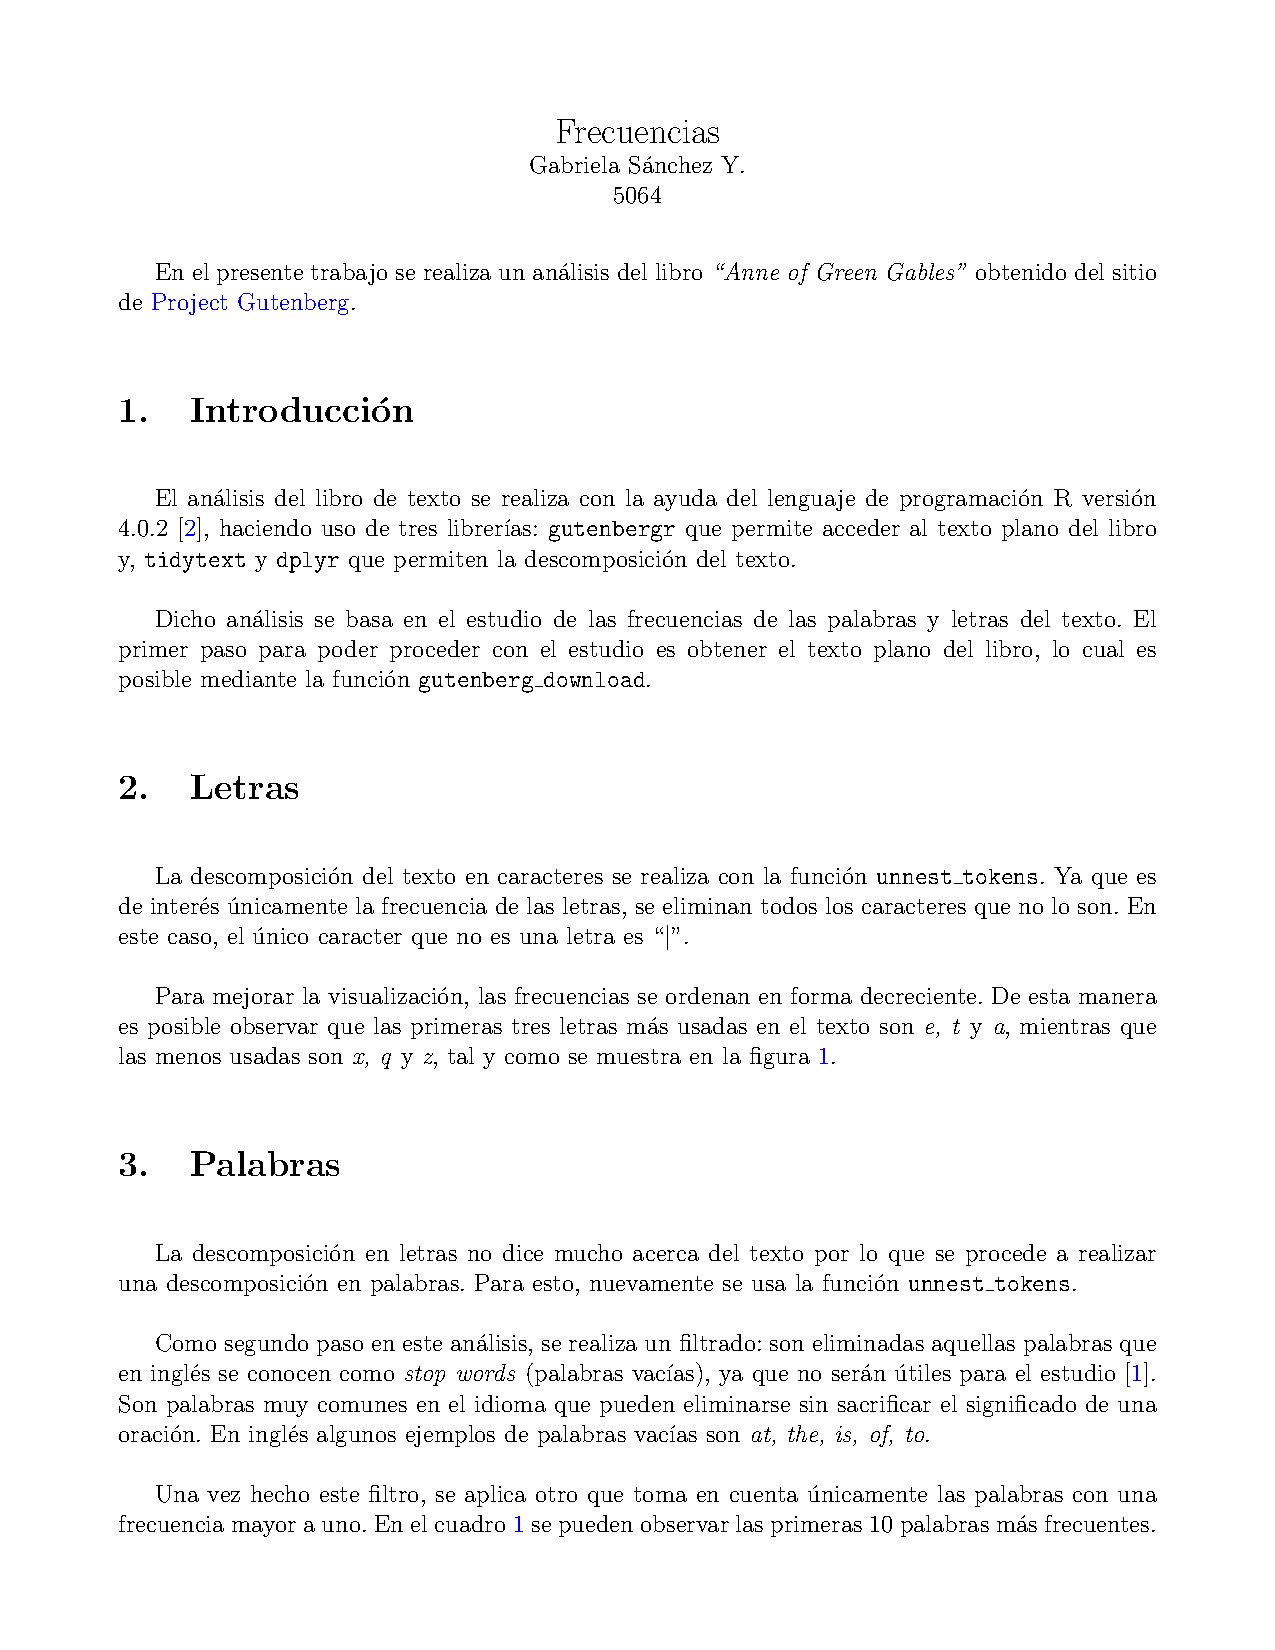
\includepdf[pages=1-5]{t2.pdf}
%%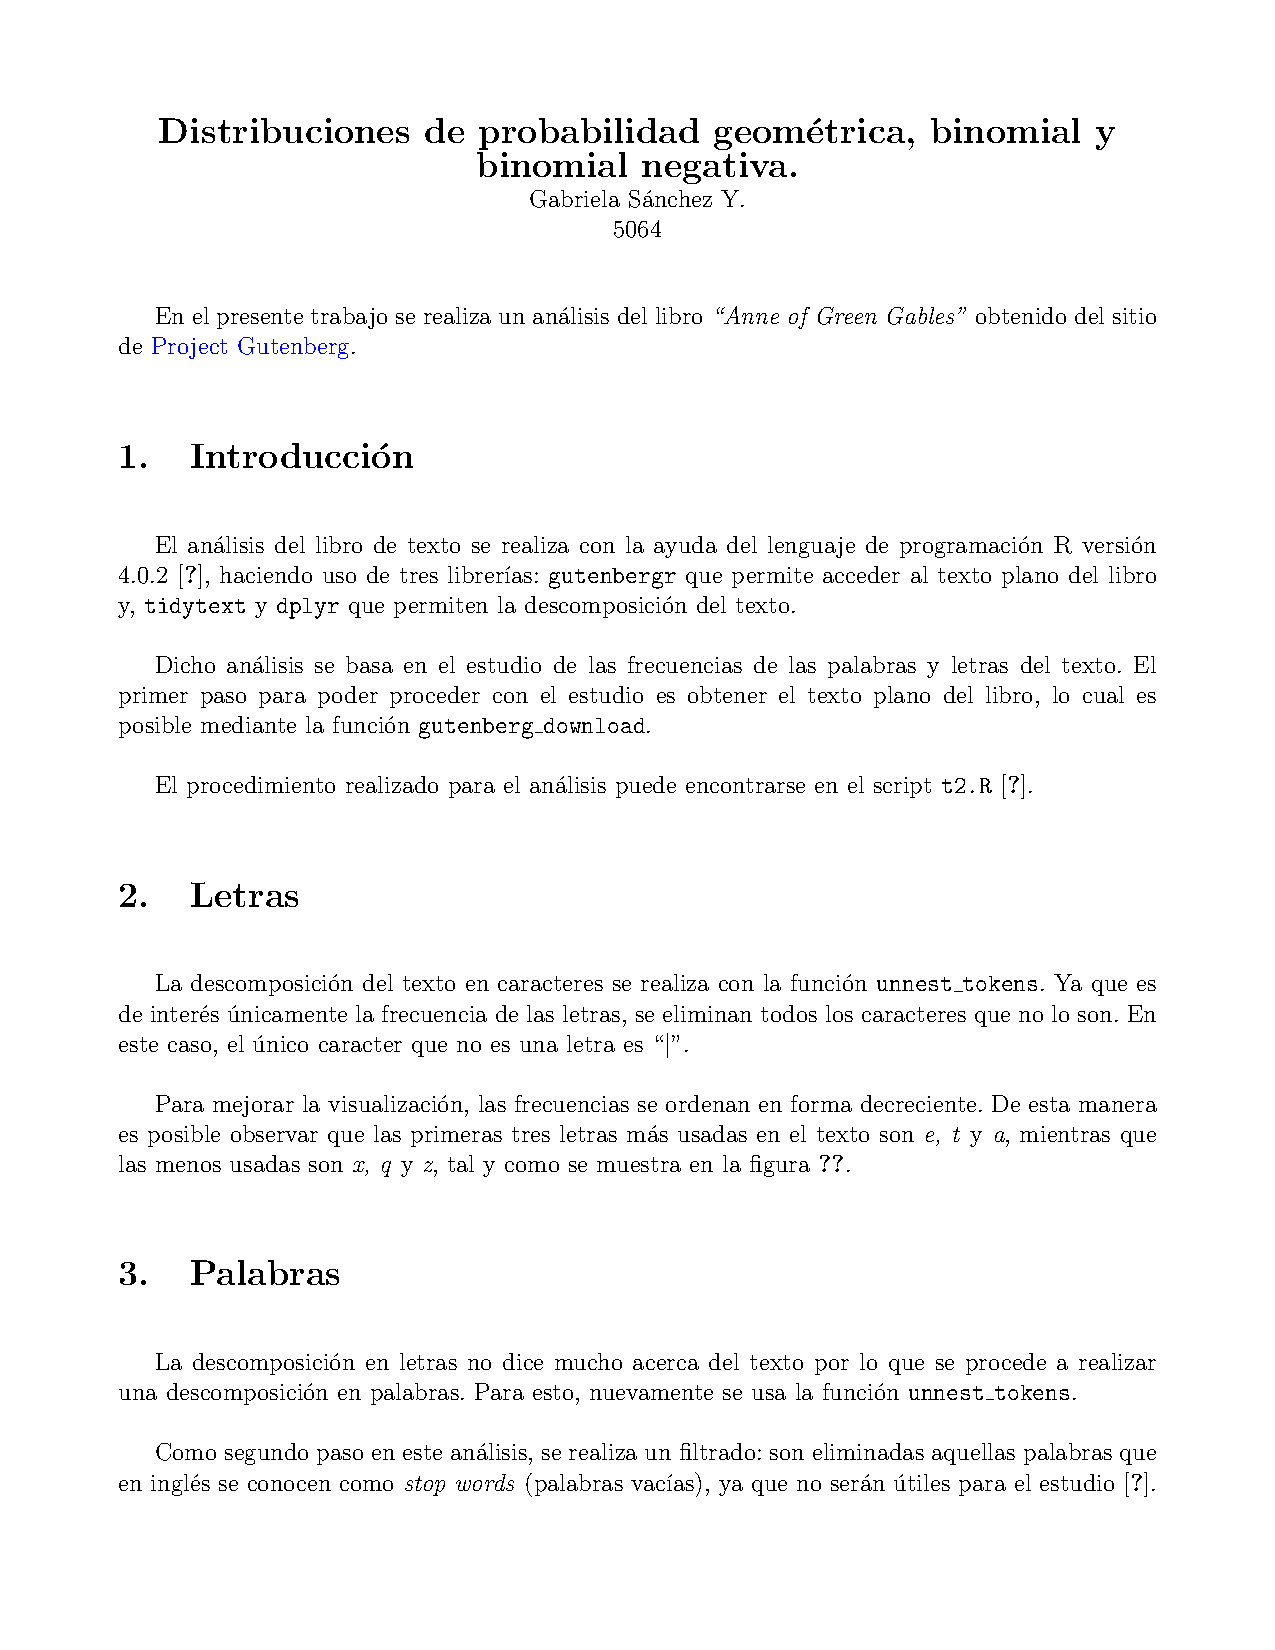
\includepdf[pages=1-5]{t3.pdf}
%%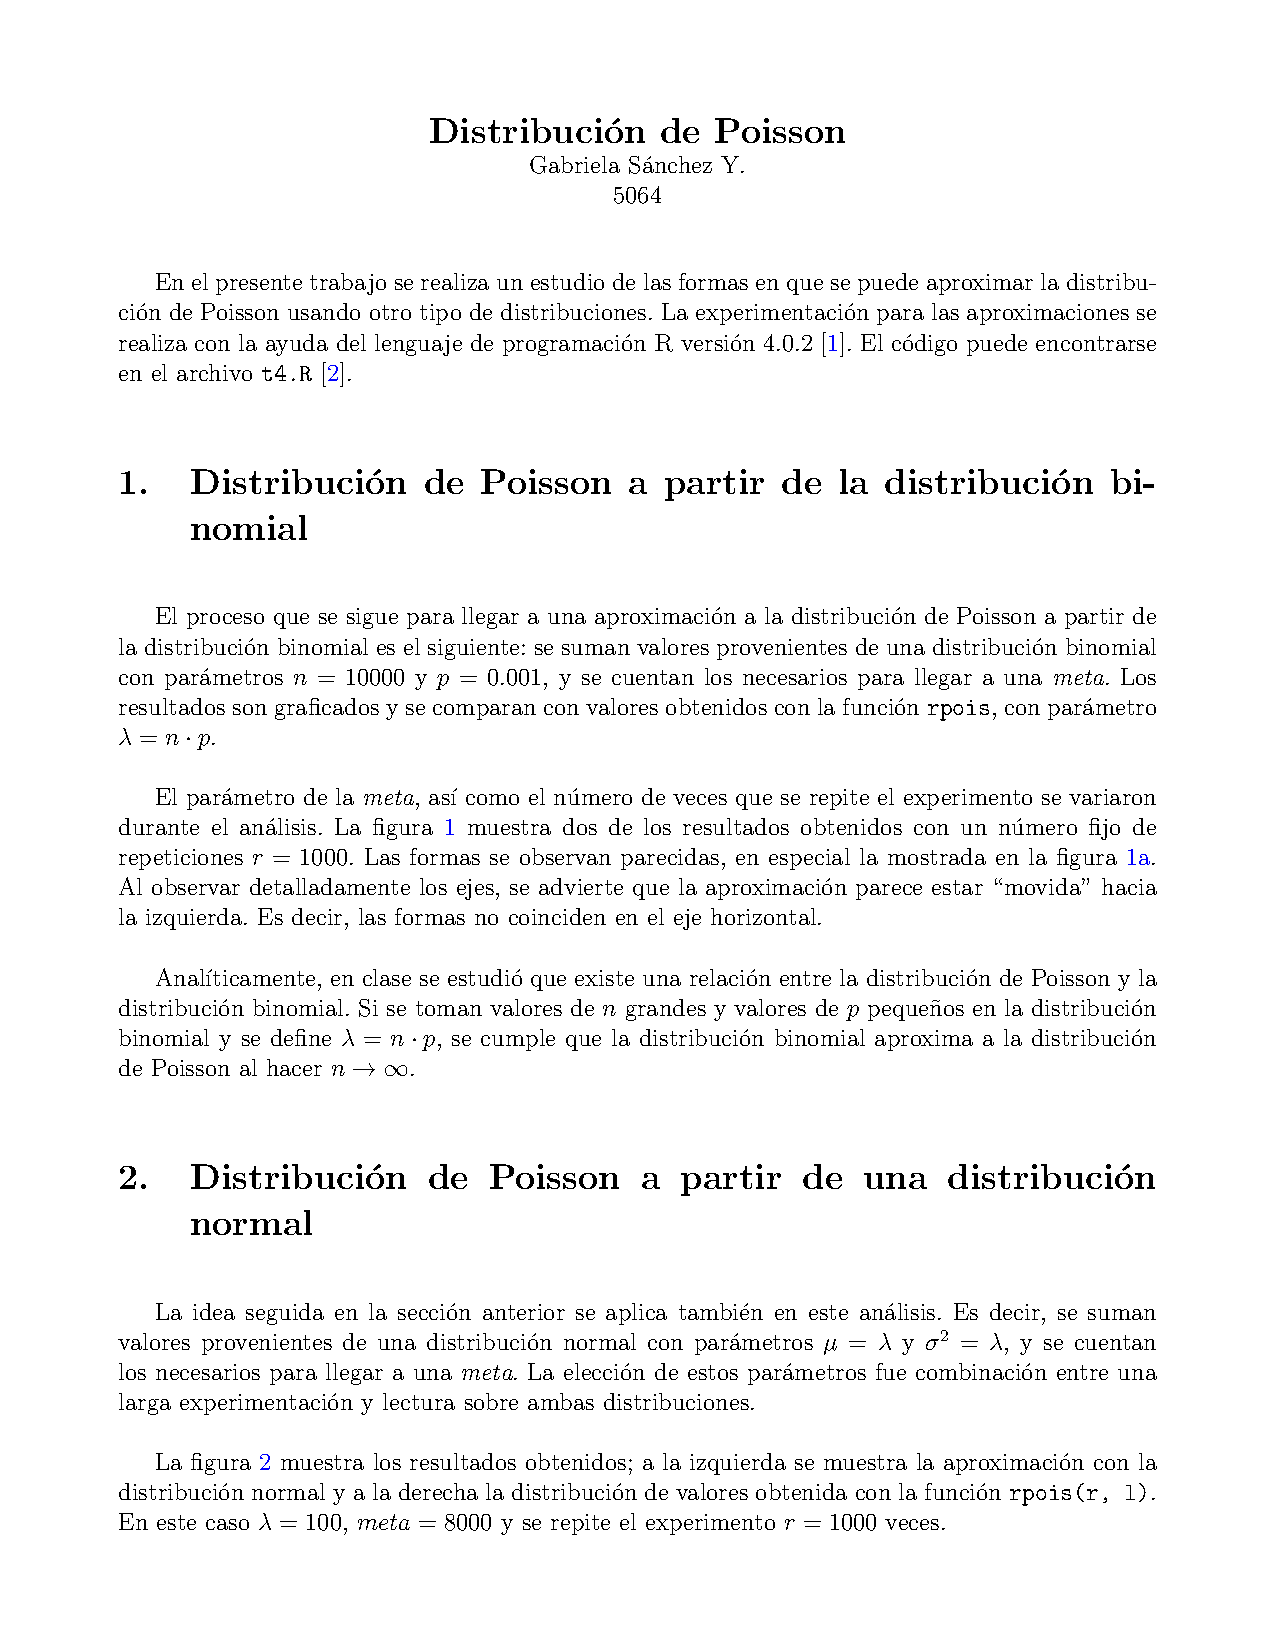
\includepdf[pages=1-5]{t4.pdf}
%%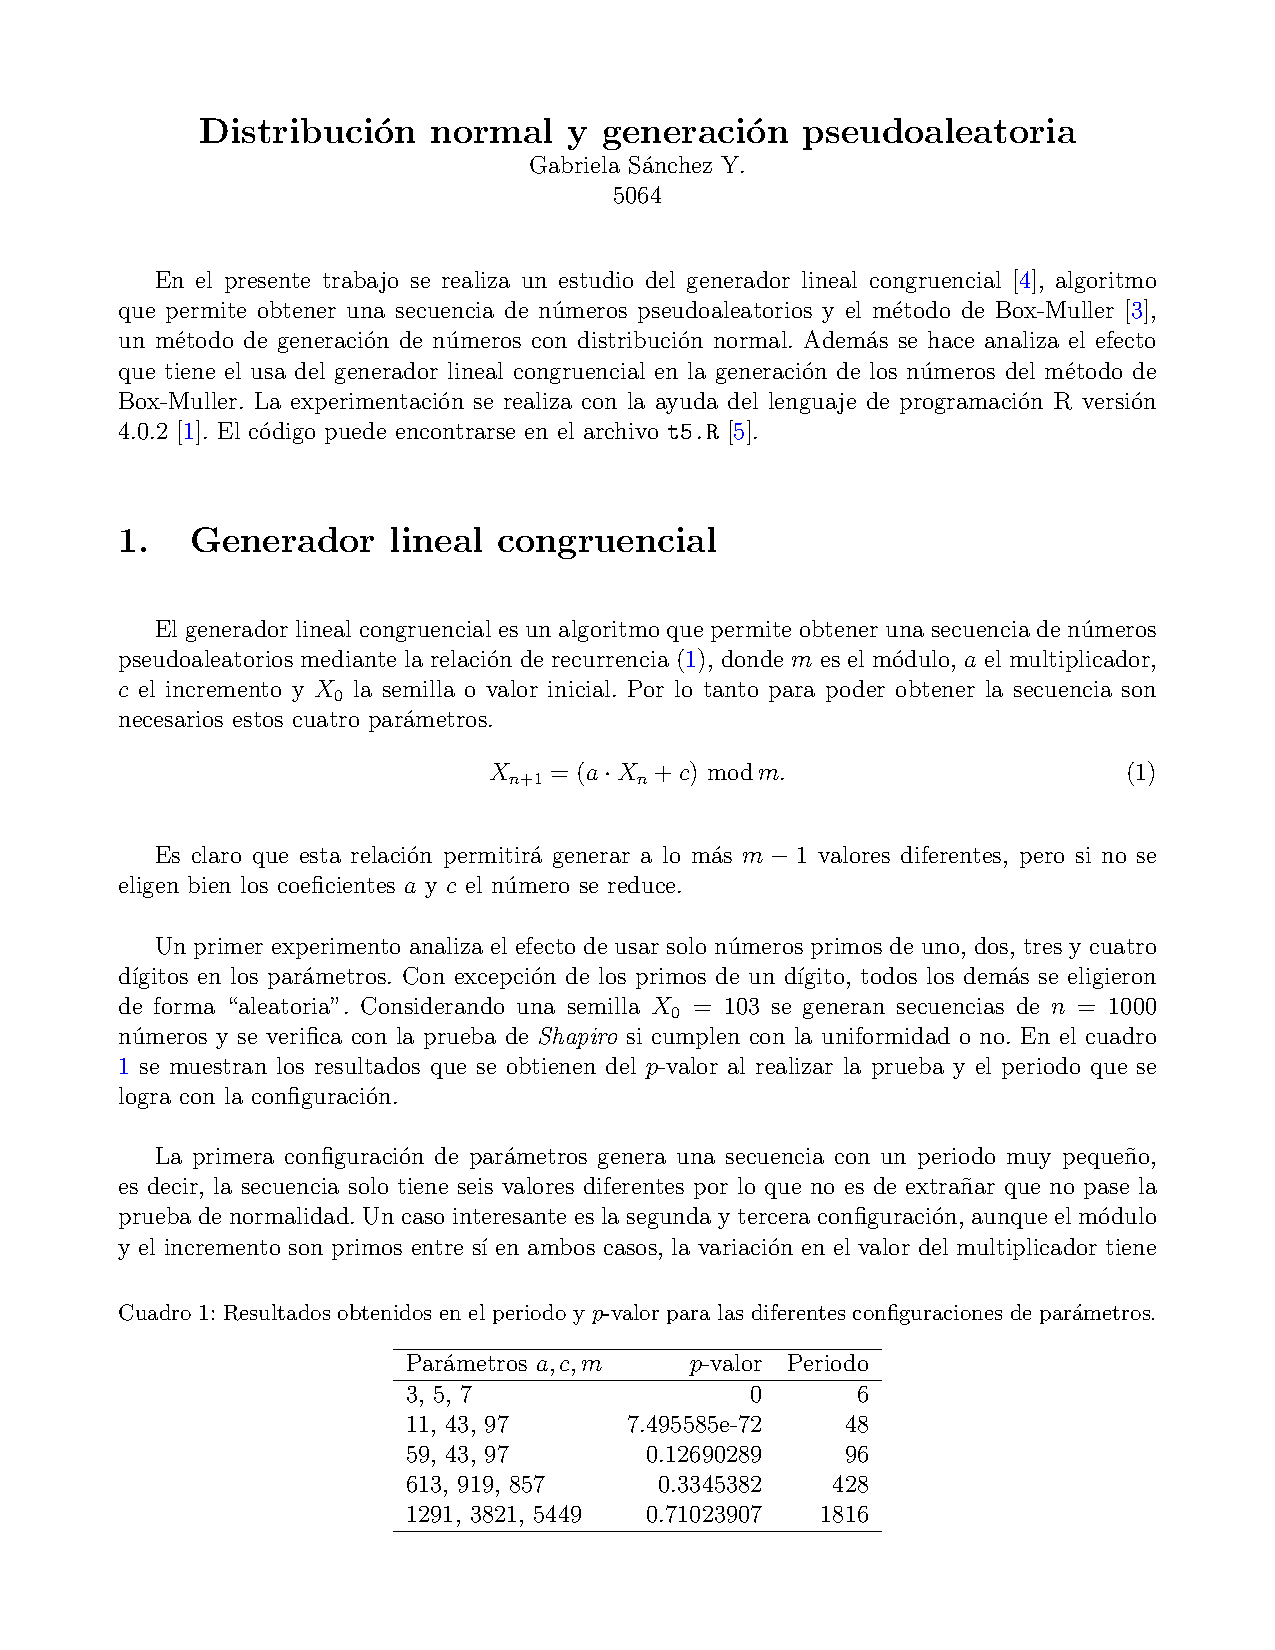
\includepdf[pages=1-8]{t5.pdf}
%%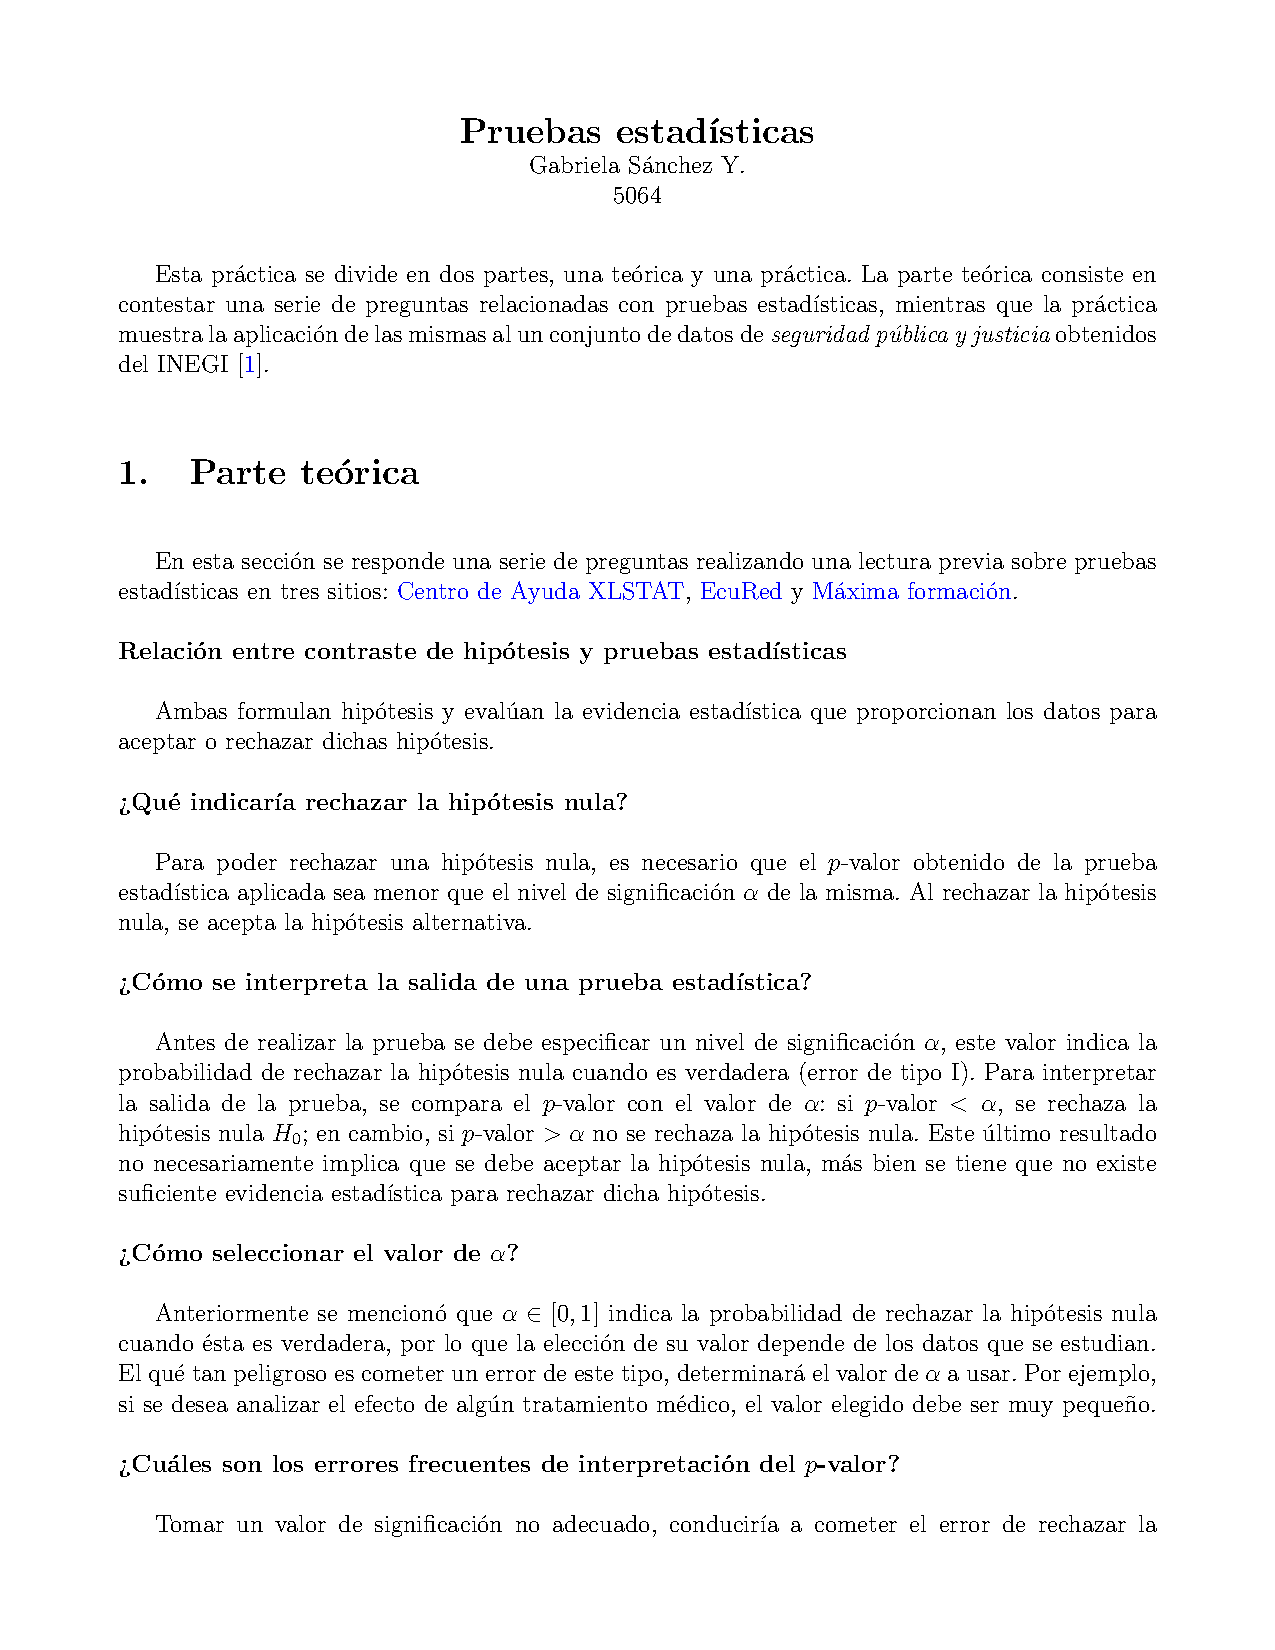
\includepdf[pages=1-8]{t6.pdf}
%%%\includepdf[pages=1-2]{7.pdf}
%%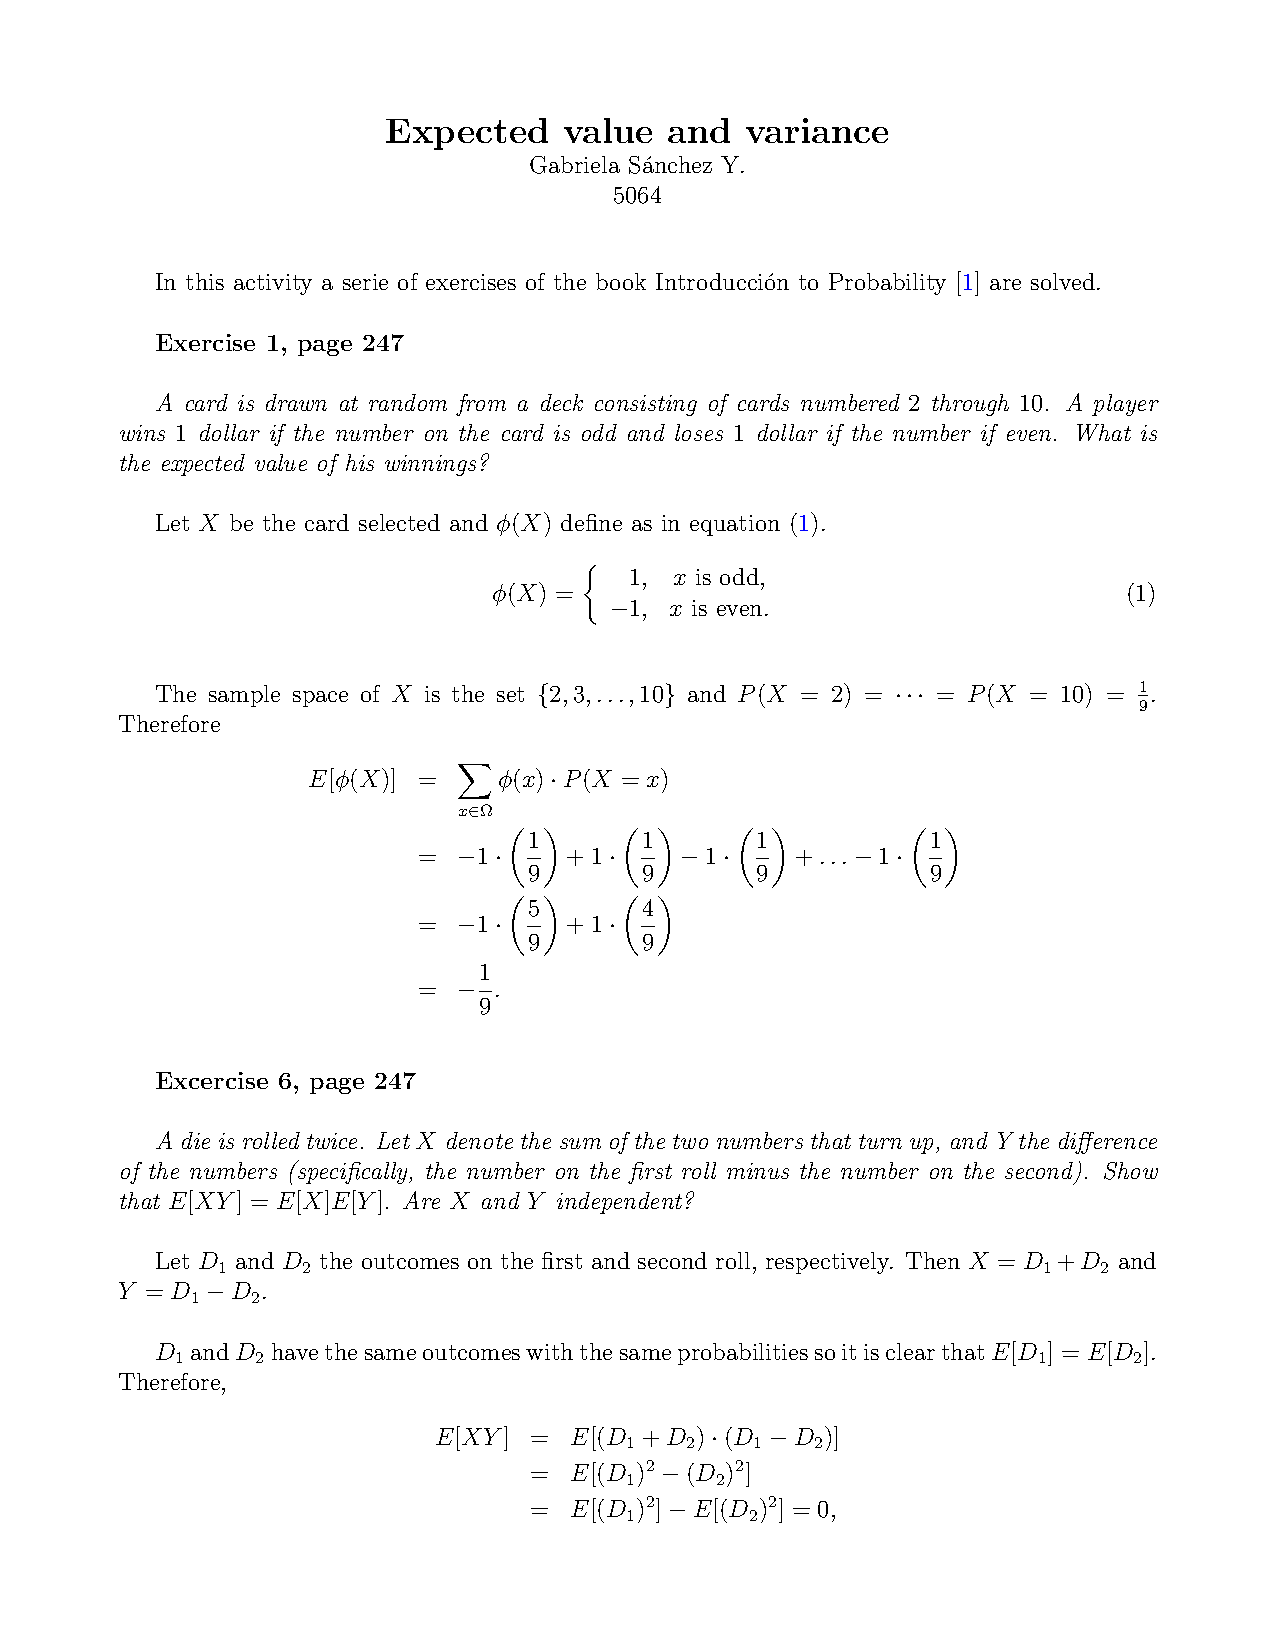
\includepdf[pages=1-9]{t9.pdf}
%%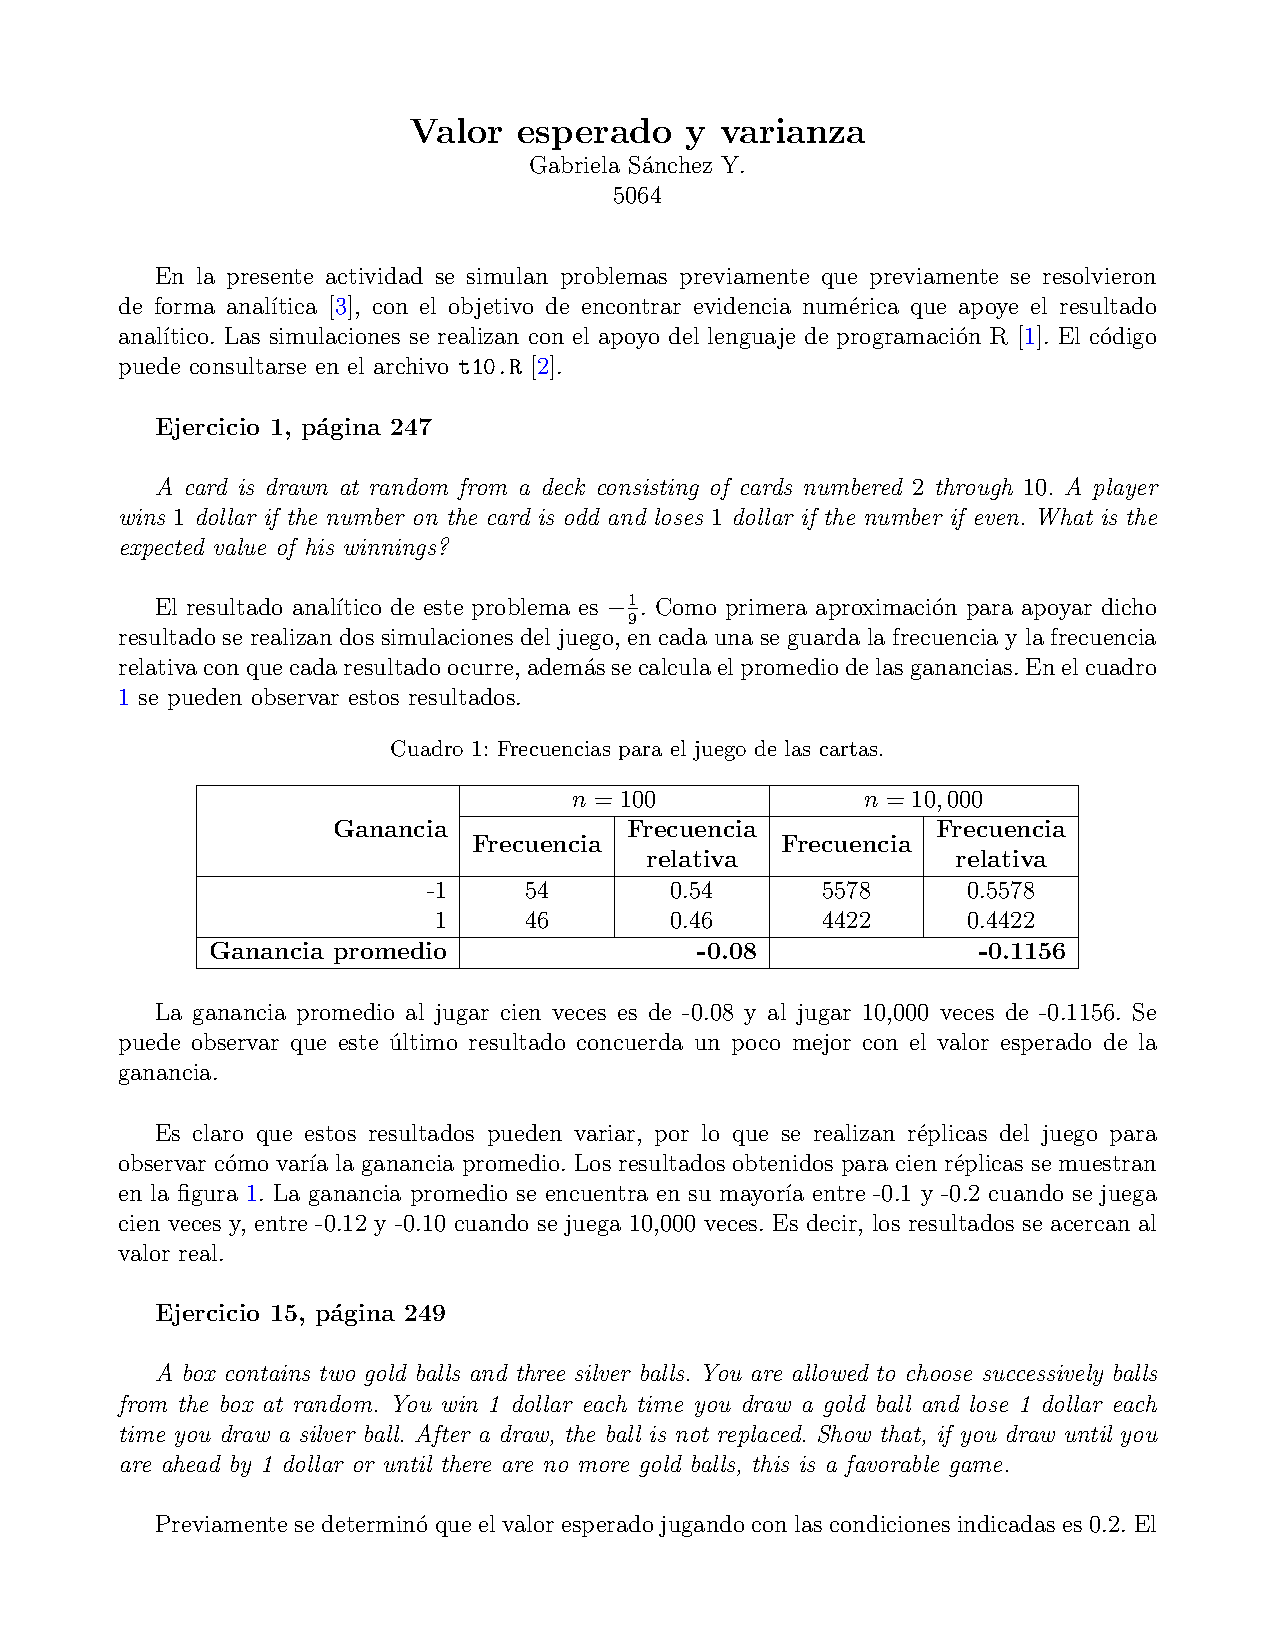
\includepdf[pages=1-5]{t10.pdf}
%%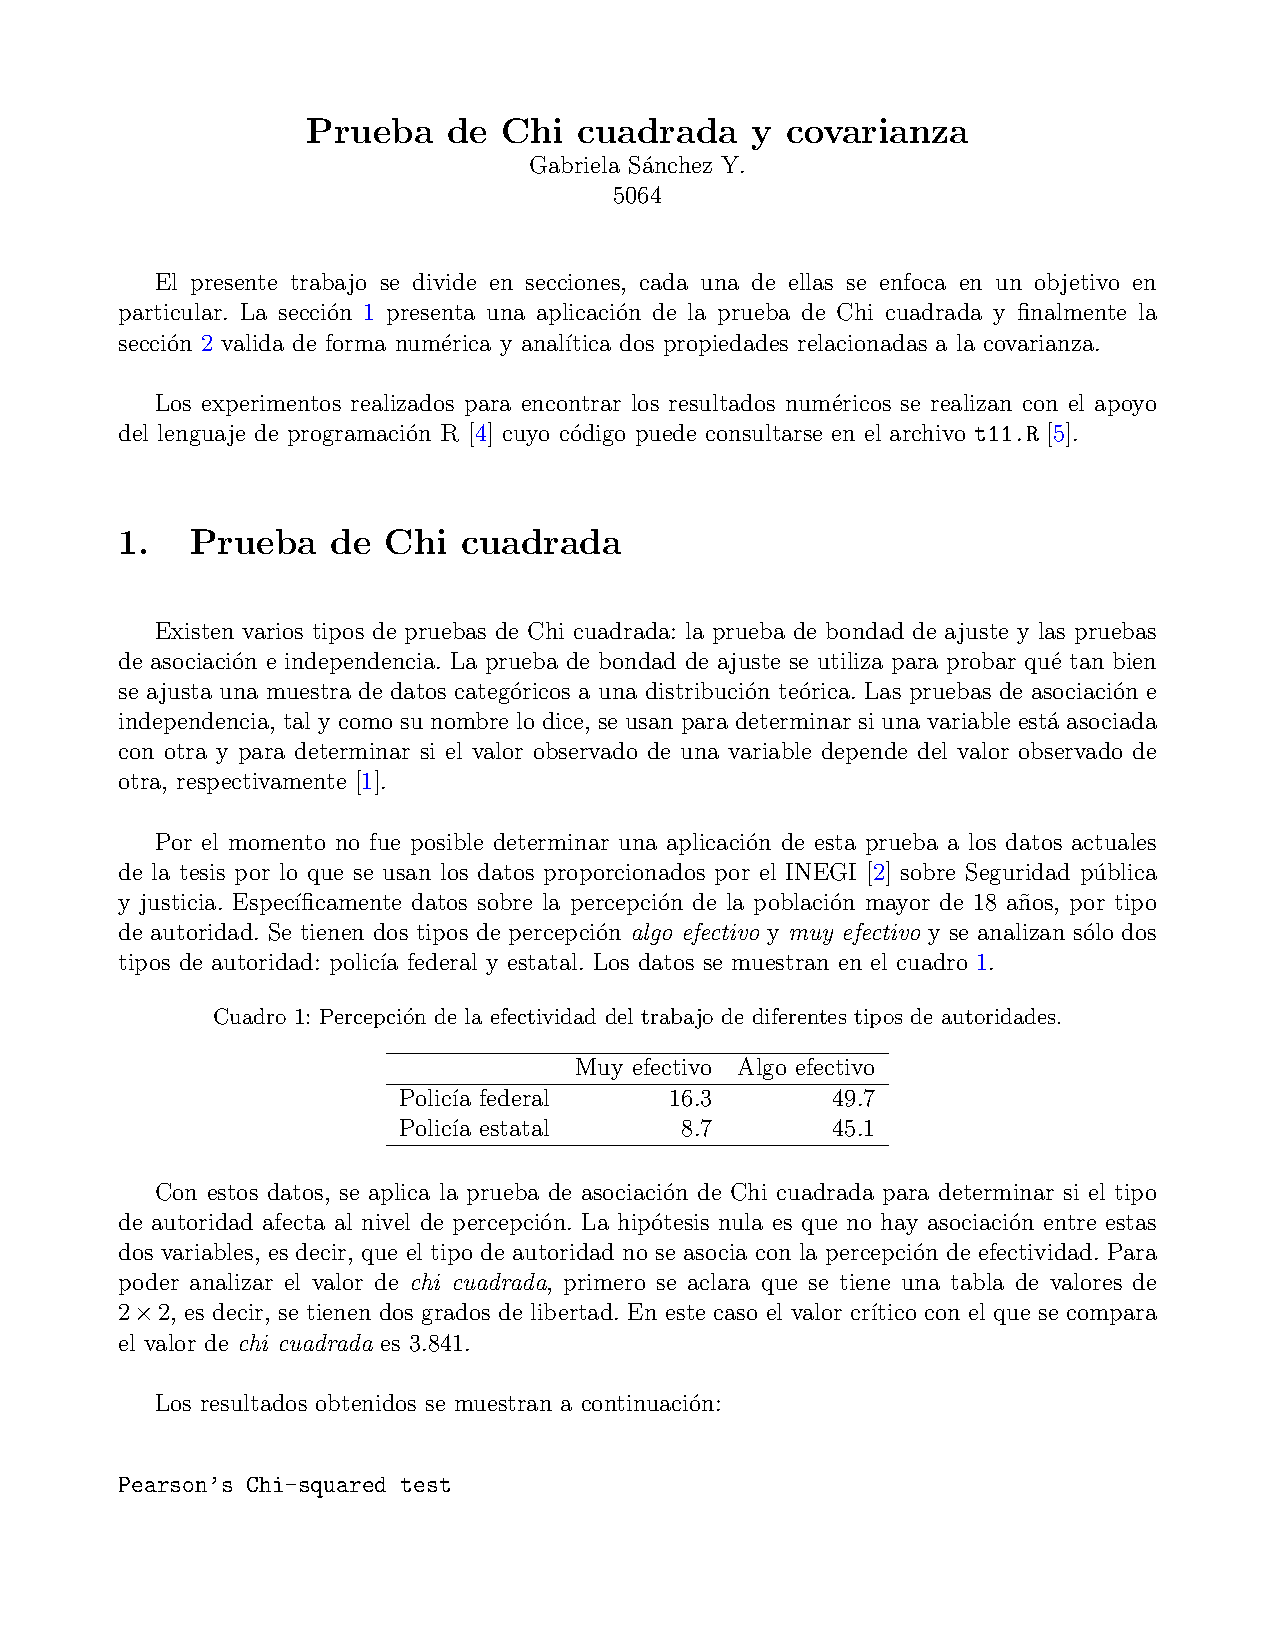
\includepdf[pages=1-5]{t11.pdf}
%%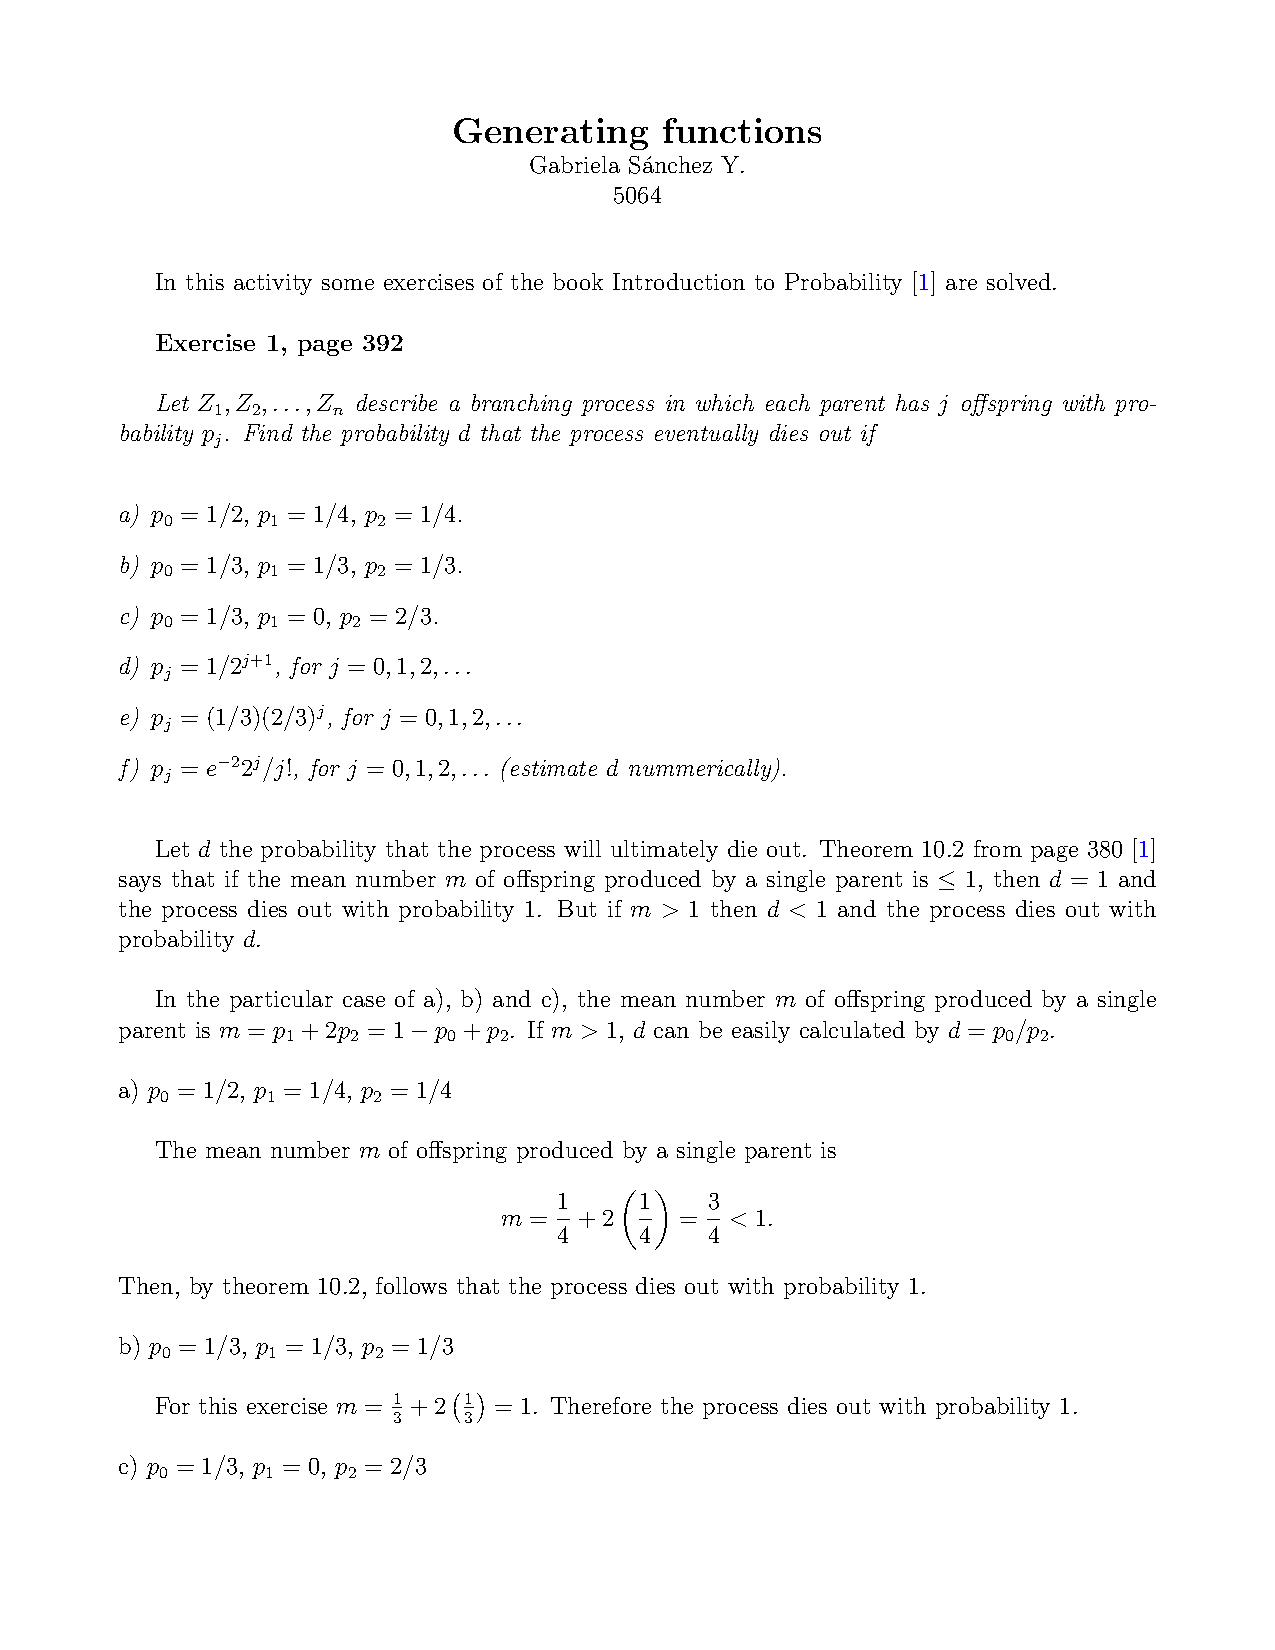
\includepdf[pages=1-7]{t12.pdf}
%%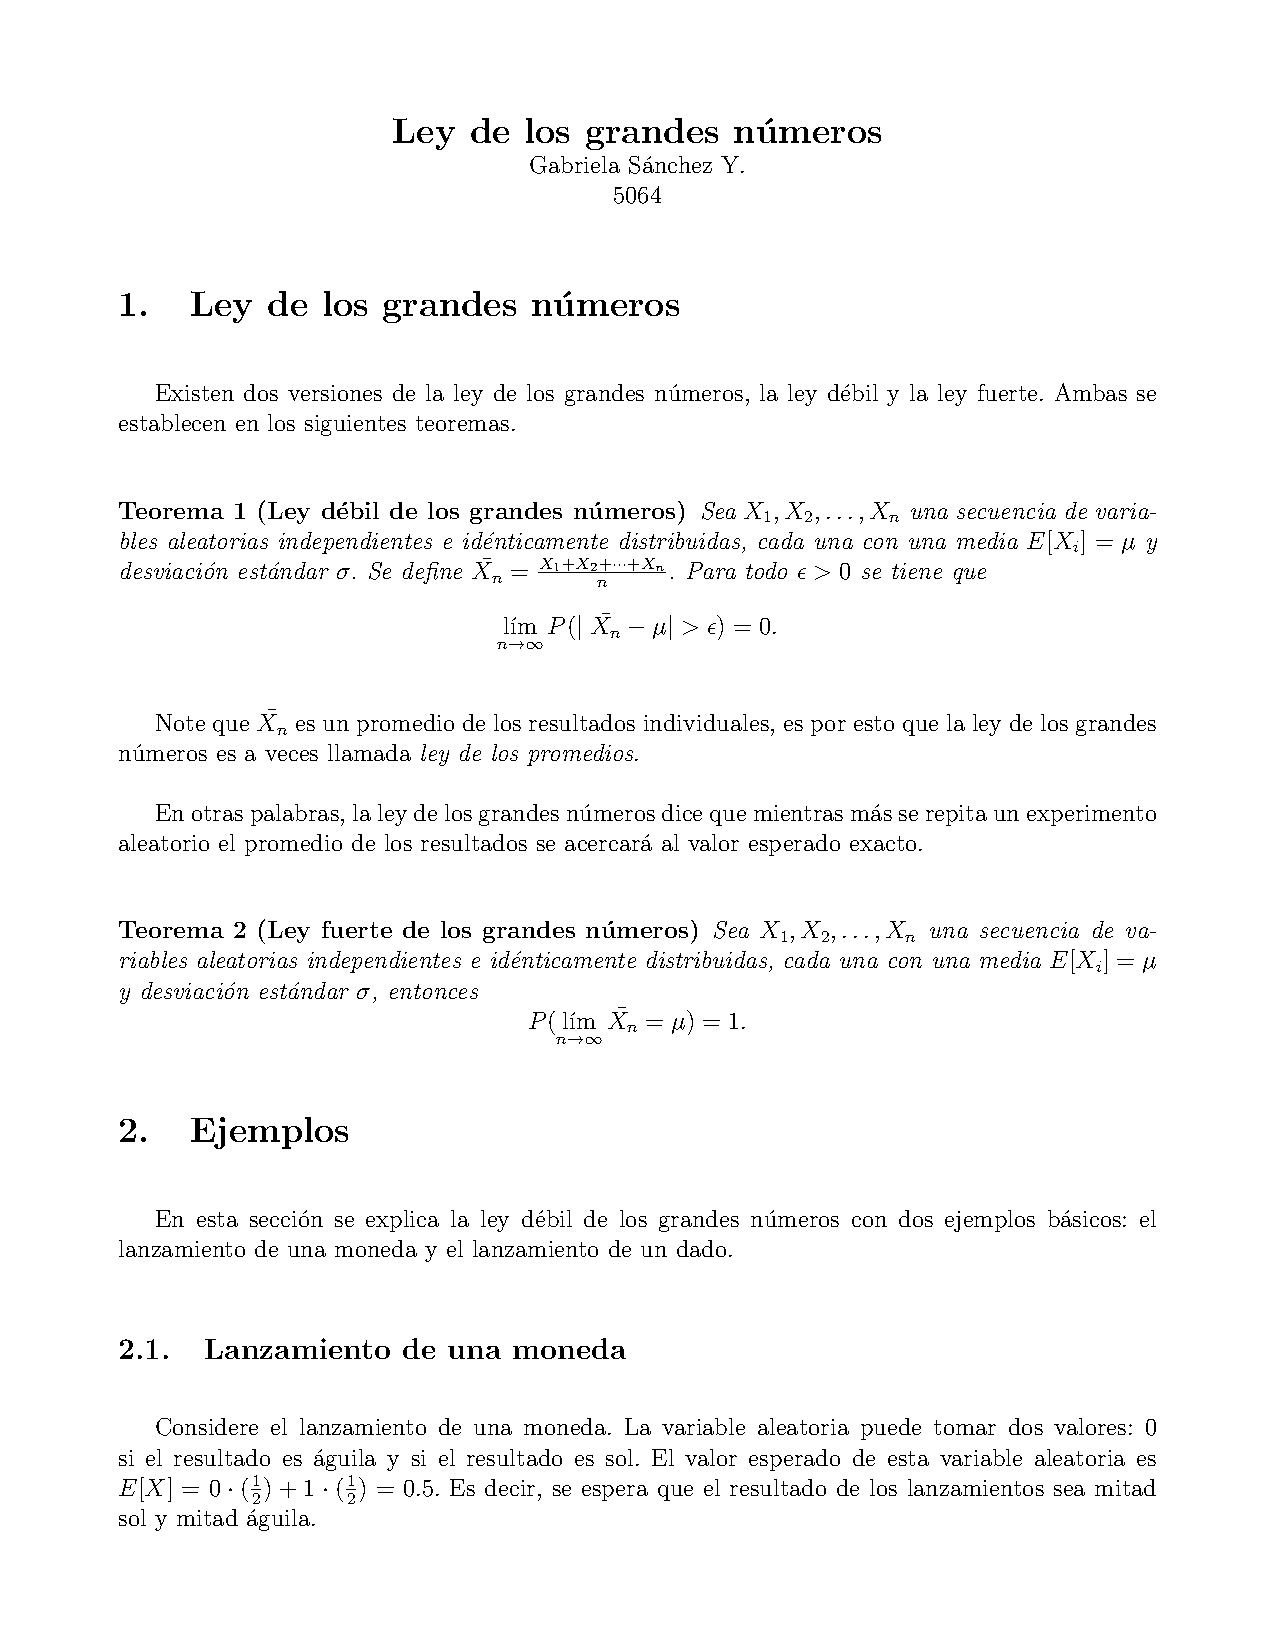
\includepdf[pages=1-3]{t13.pdf}
%%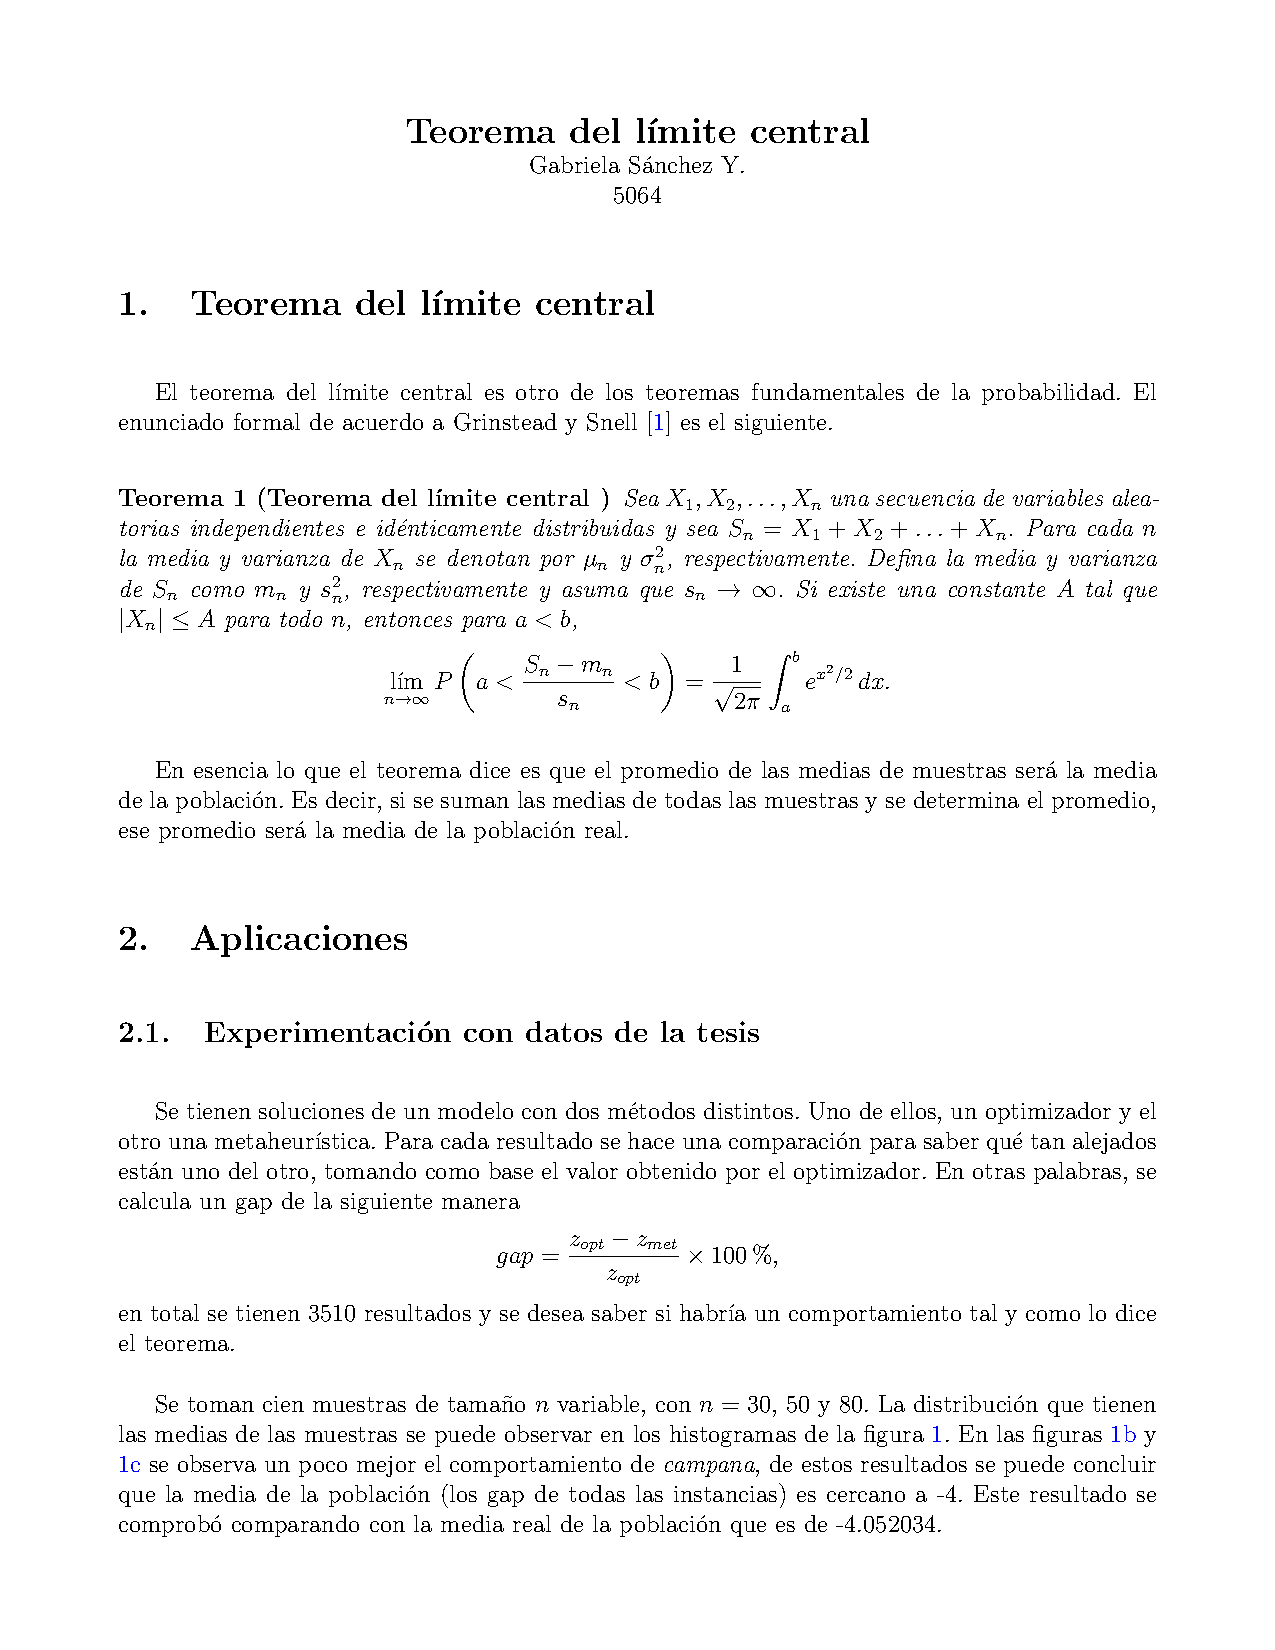
\includepdf[pages=1-3]{t14.pdf}
%%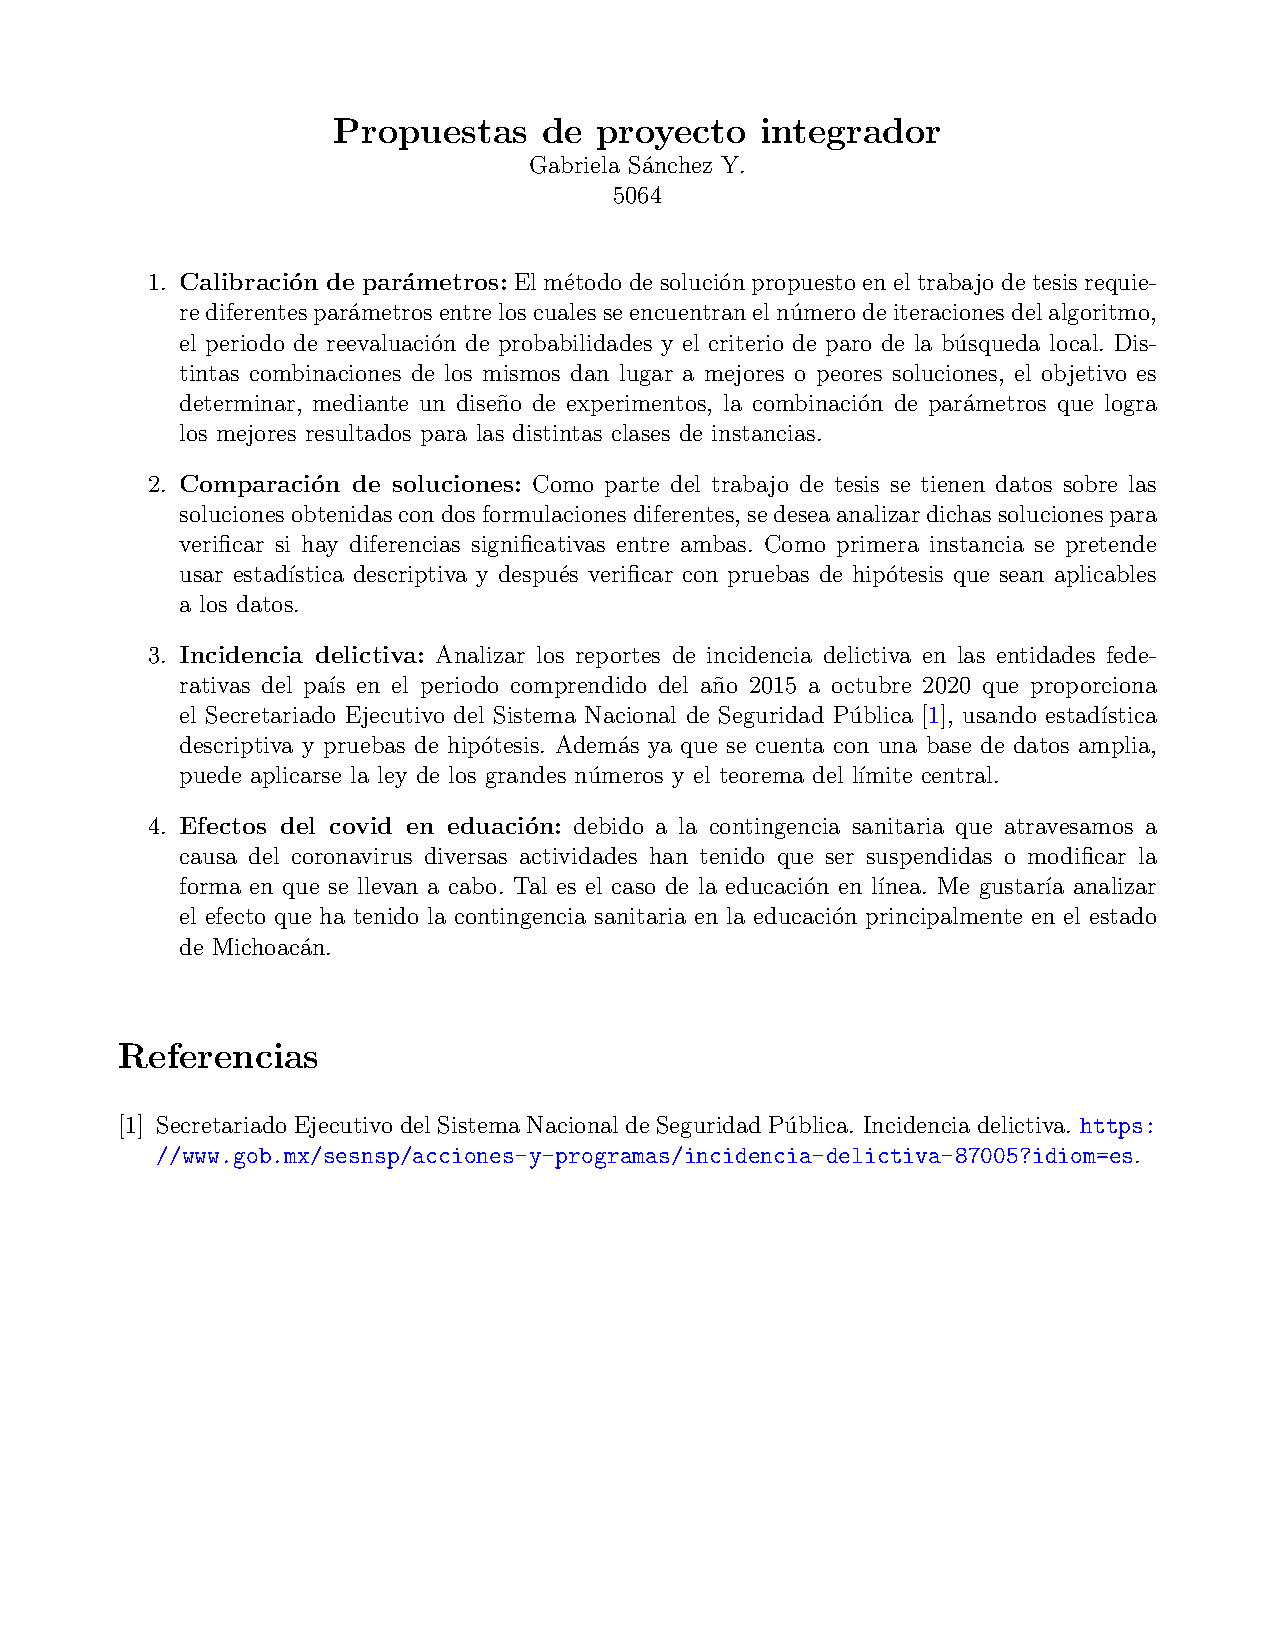
\includepdf[pages=1-1]{t15.pdf}
%%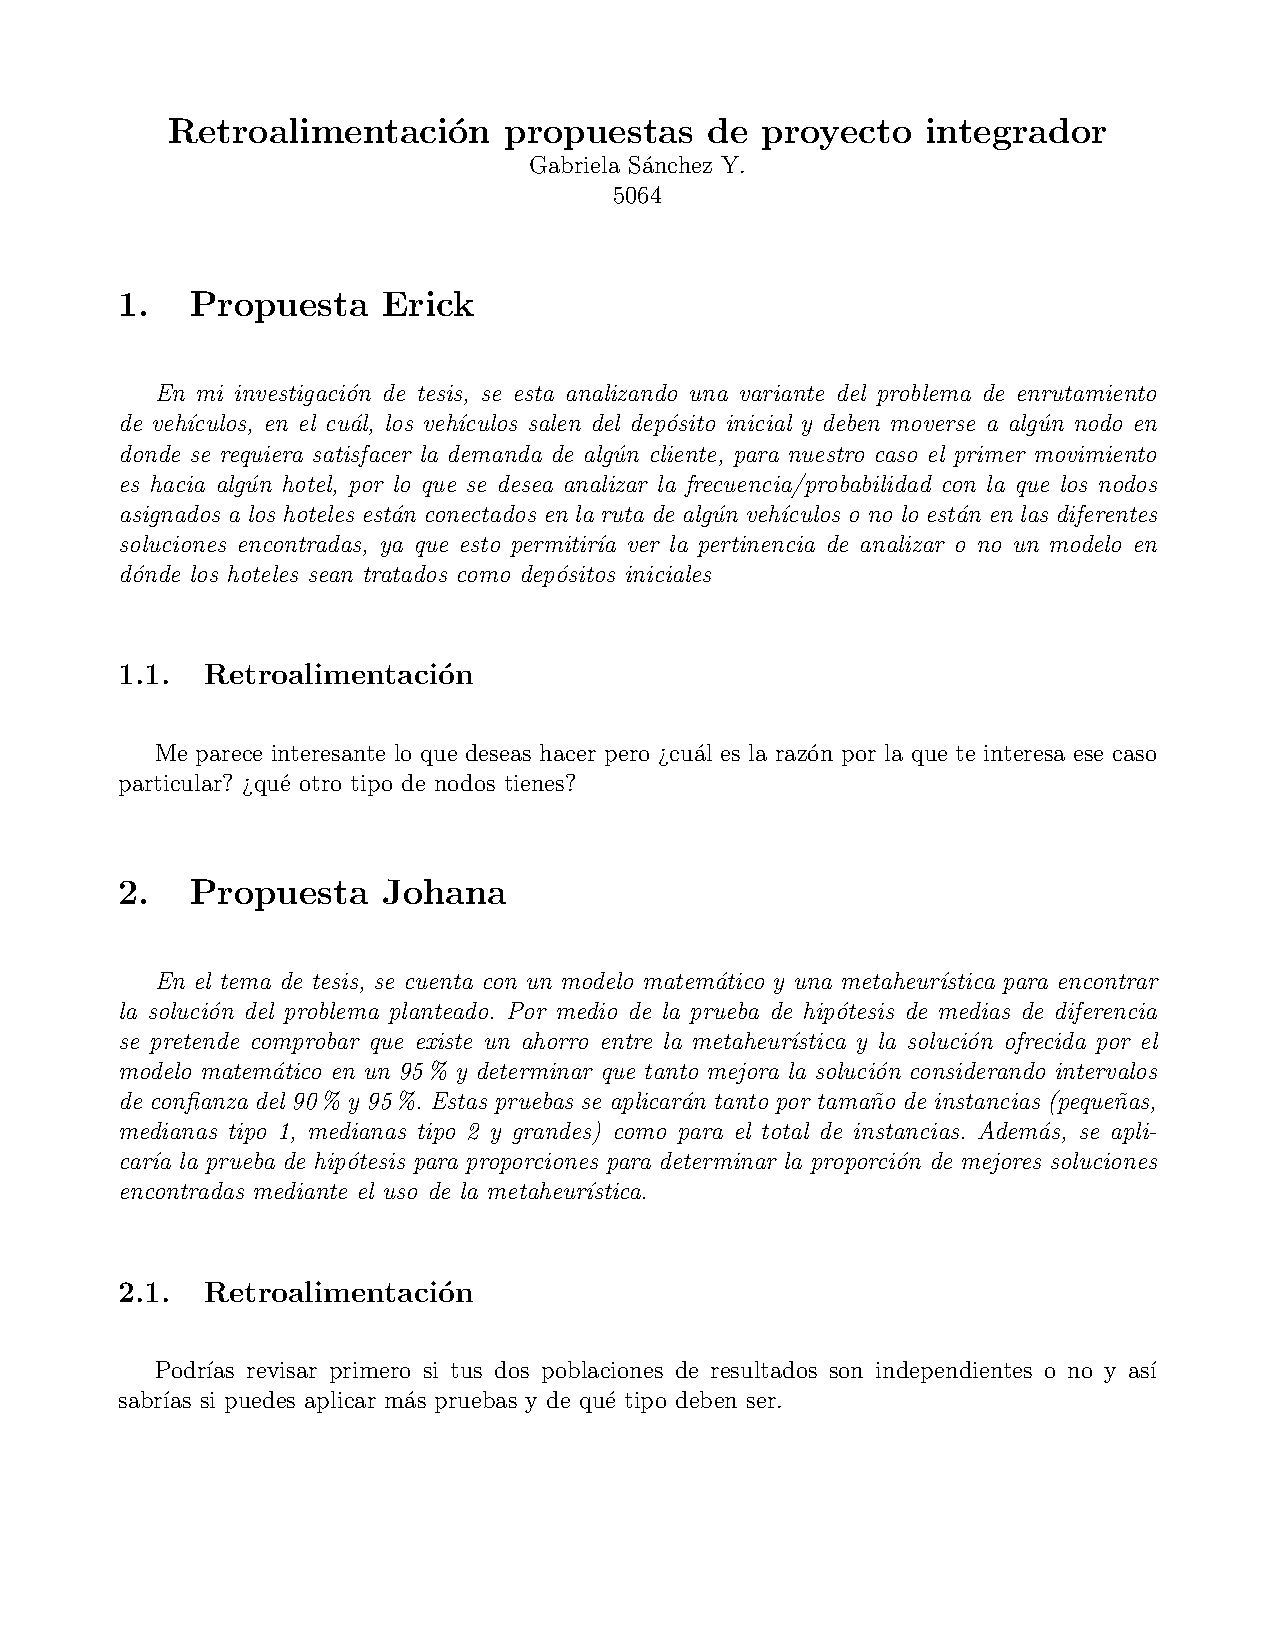
\includepdf[pages=1-2]{t16.pdf}
%%	
%\end{document}


\documentclass[openany]{book}
\usepackage[utf8]{inputenc}
\usepackage{pdfpages}
\usepackage{hyperref, subcaption}
\usepackage[spanish]{babel}

\begin{document}
	
	\frontmatter
	\thispagestyle{empty}
\begin{scshape}
\begin{center}
	{\Large{Universidad Autónoma de Nuevo León}} \\[5mm]
	{\large{Facultad de Ingeniería Mecánica y Eléctrica}} \\[5mm]
	{\large{Posgrado en Ingeniería de Sistemas}} \\[5 mm]
	{\large{Doctorado}}
	\vskip16mm
	\begin{figure}[h!]
		\centering
		\begin{subfigure}{0.3\linewidth}
			\includegraphics[width=\linewidth]{images/uanl}
		\end{subfigure}
		\hspace{15 mm}
		\begin{subfigure}{0.2\linewidth}
			\includegraphics[width=\linewidth]{images/fime}
		\end{subfigure}
	\end{figure}
	\vskip16mm
	\begin{tabular}{p{11cm}}
		\centering
		{\large Portafolio de Evidencias}
	\end{tabular}
	\vskip7mm
	{de}\\[7mm]
	{\large Gabriela Sánchez Yepez}\\[3mm]
	{1935064}\\[7 mm]
	{para el curso de Modelos Probabilistas Aplicados,}\\[3mm]
	{con la profesora Dra. Satu Elisa Schaeffer.}\\[3mm]
	Semestre Agosto 2020 - Enero 2021. \\ [5 mm]
	\url{https://github.com/Saphira3000/MPA}
	\vfill
\end{center}
\end{scshape}
	\tableofcontents
	\mainmatter
	\clearpage
	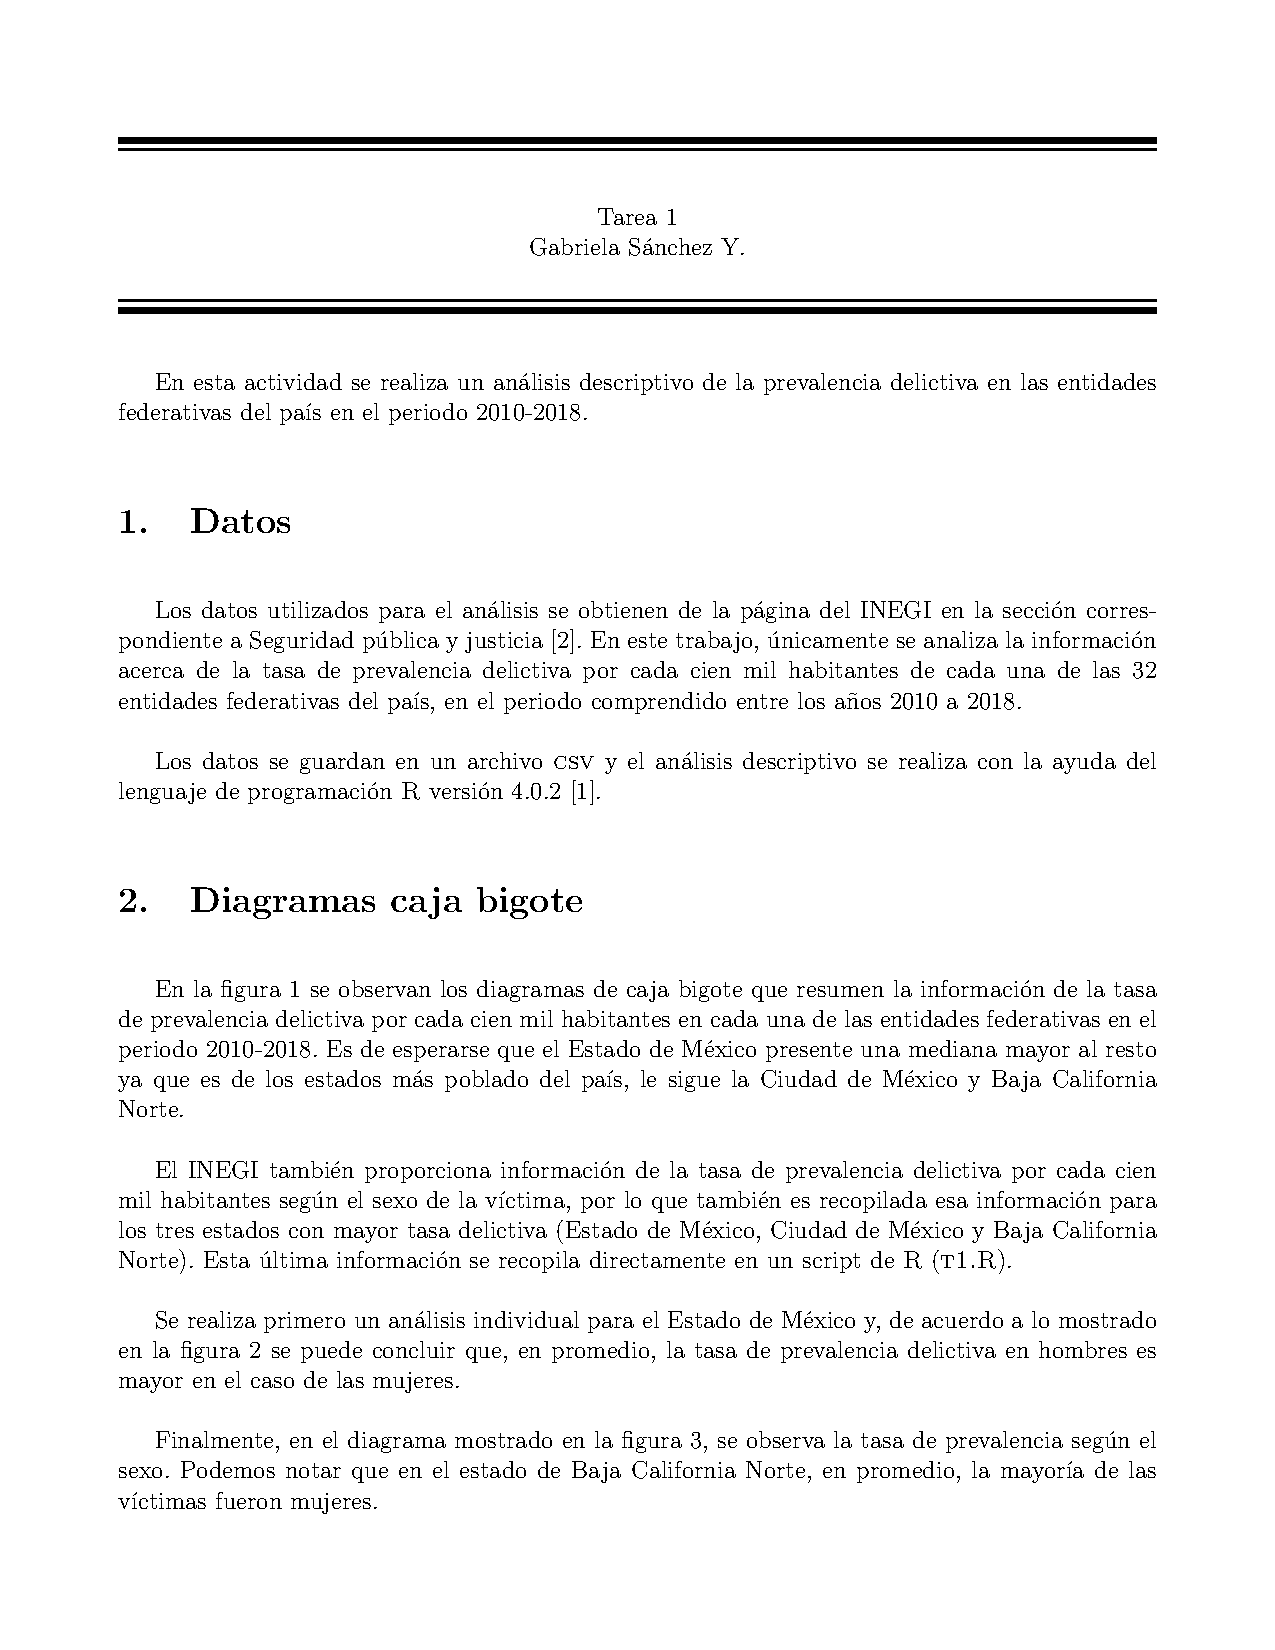
\includepdf[pages=-, addtotoc={1,chapter,1,{Tarea 1: Diagramas caja bigote}, t1}]{t1.pdf}
	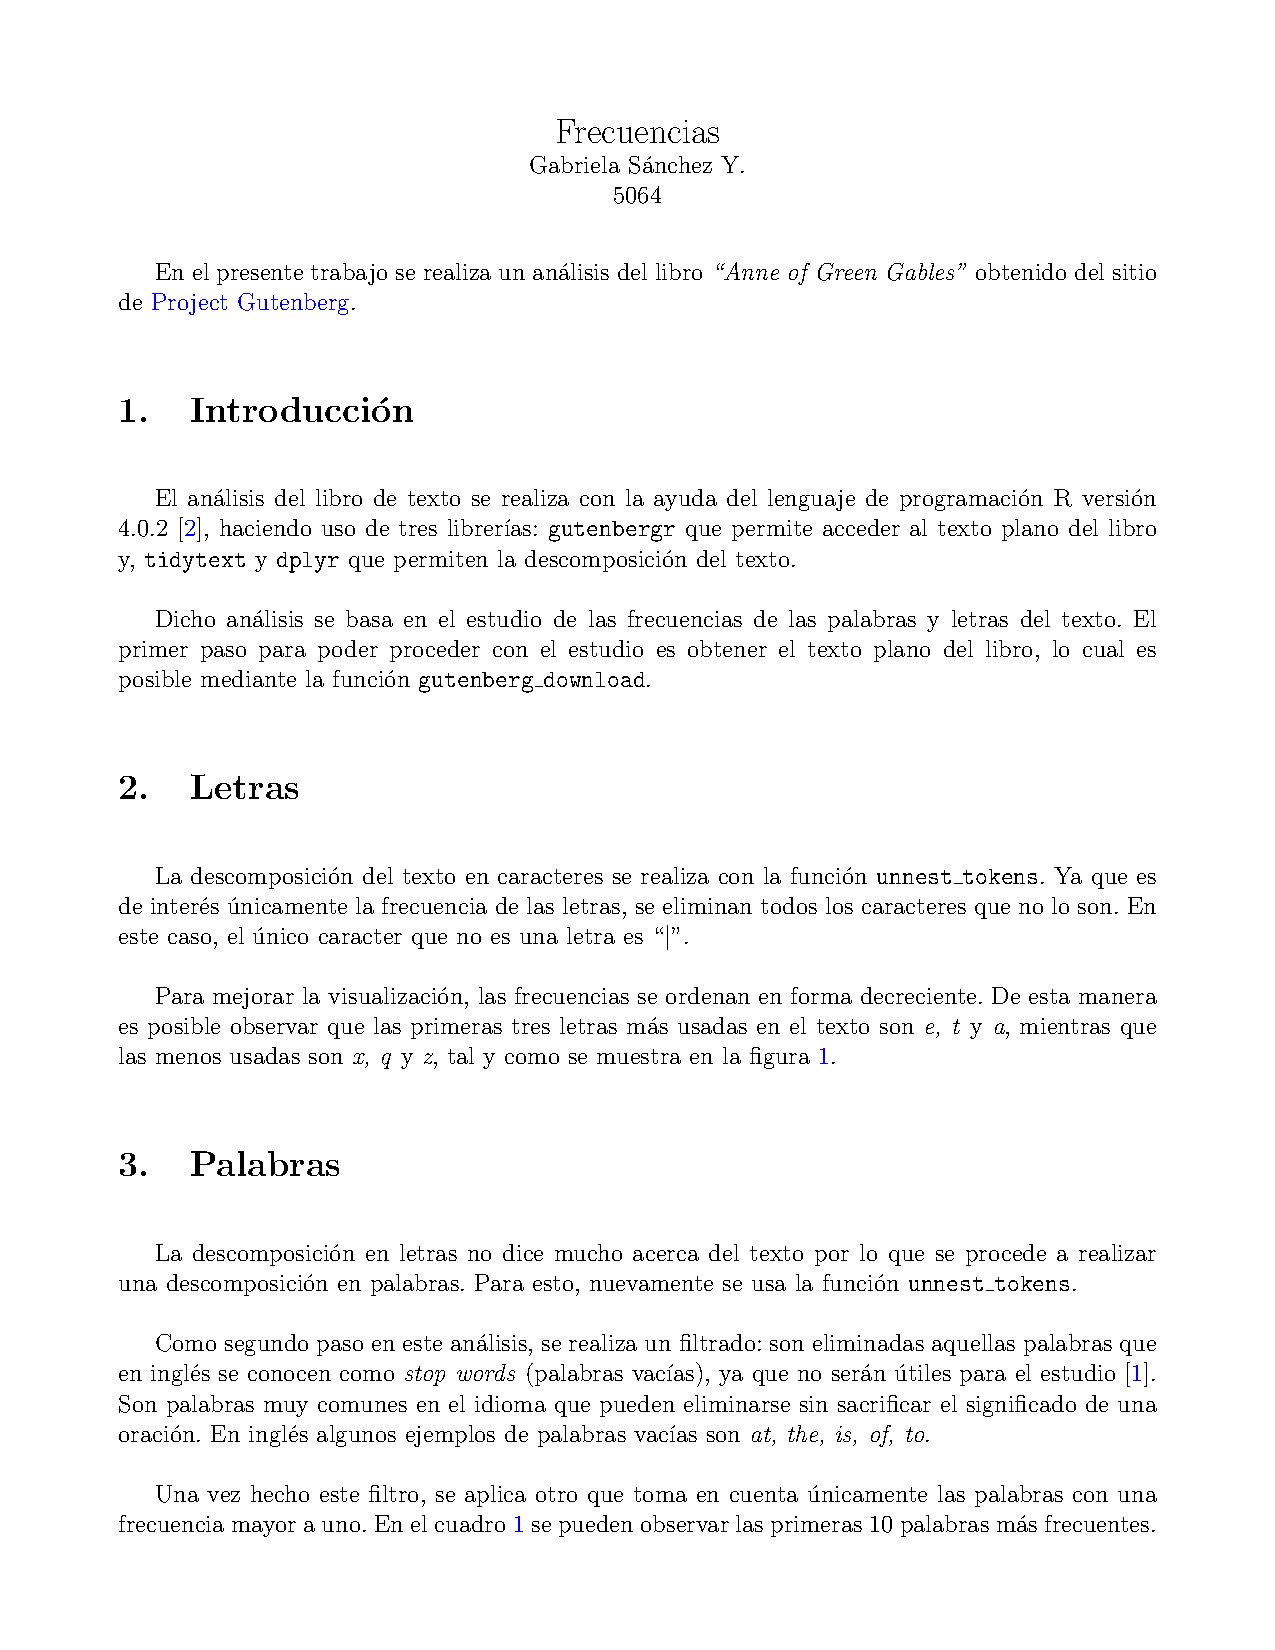
\includepdf[pages=-, addtotoc={1,chapter,2,{Tarea 2: Frecuencias}, t2}]{t2.pdf}
	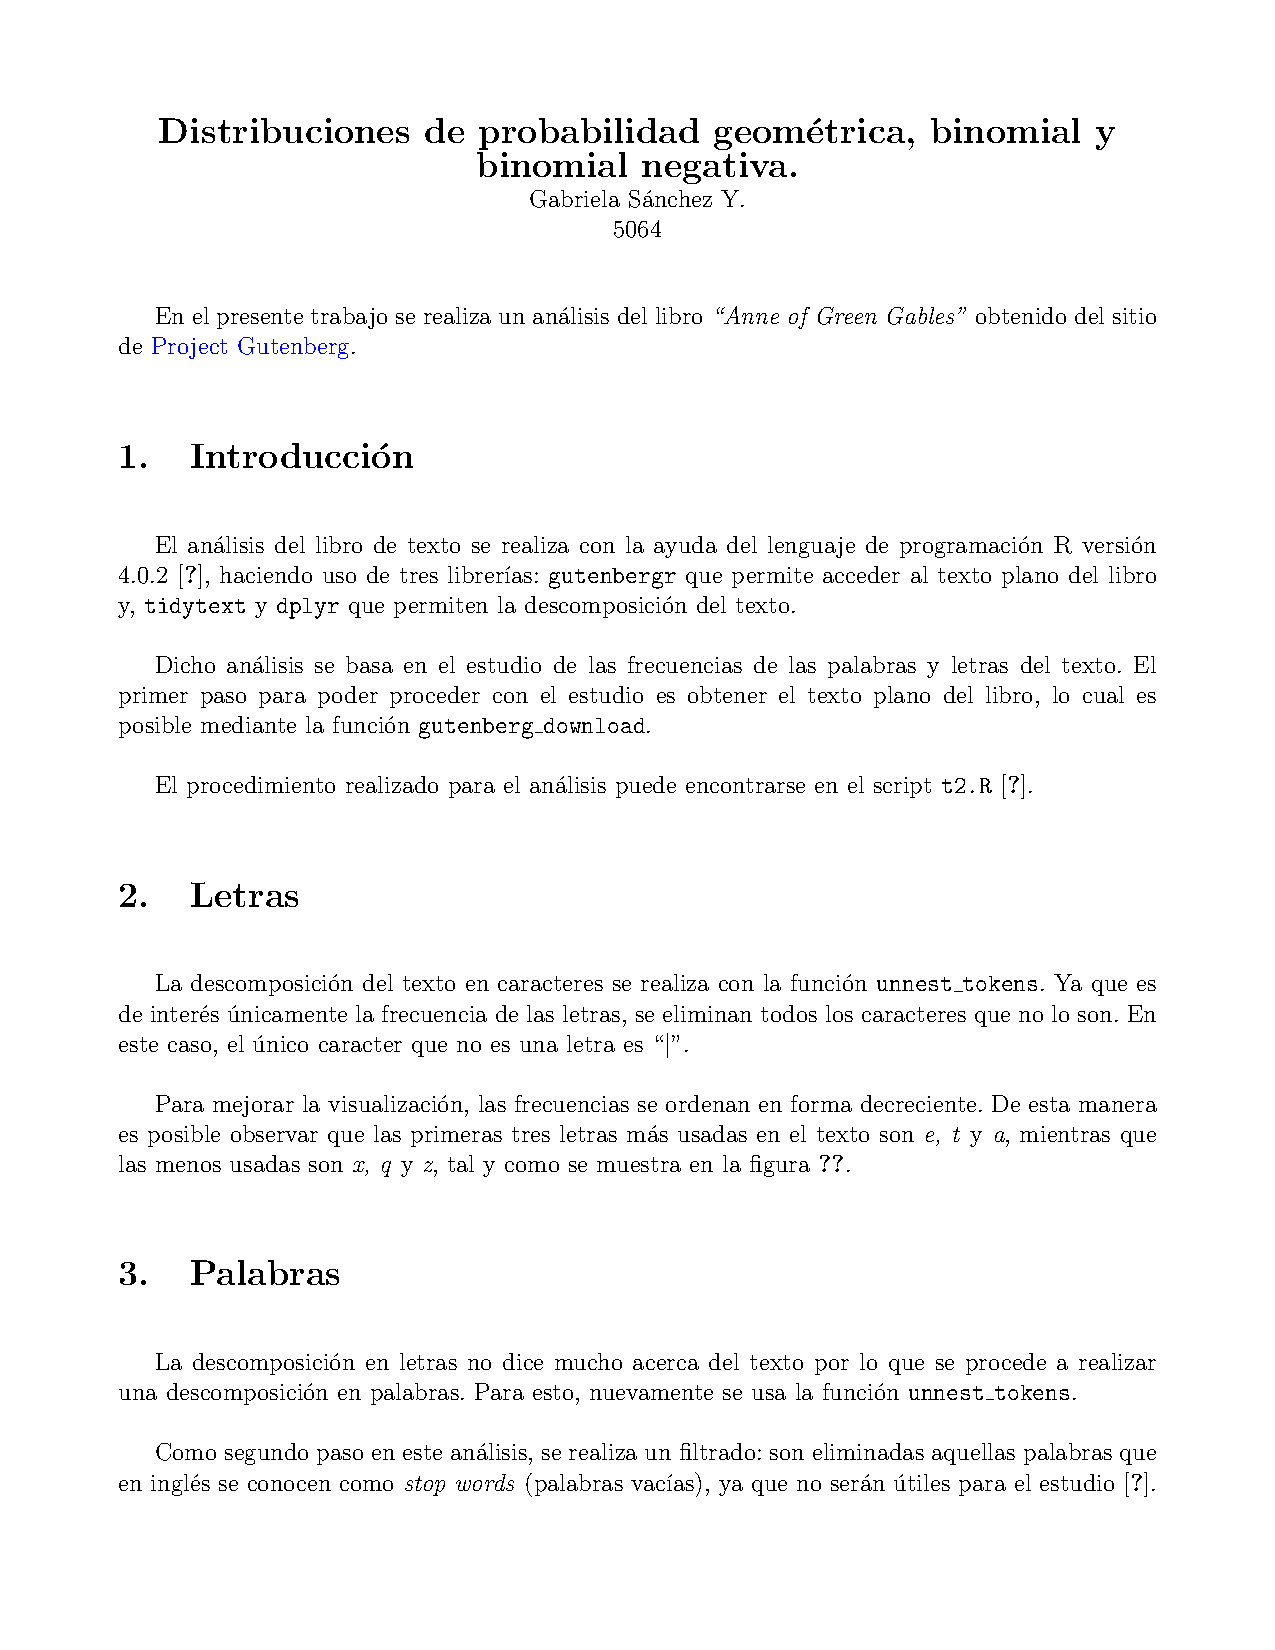
\includepdf[pages=-, addtotoc={1,chapter,3,{Tarea 3: Distribuciones de probabilidad geométrica, binomial y binomial negativa}, t3}]{t3.pdf}
	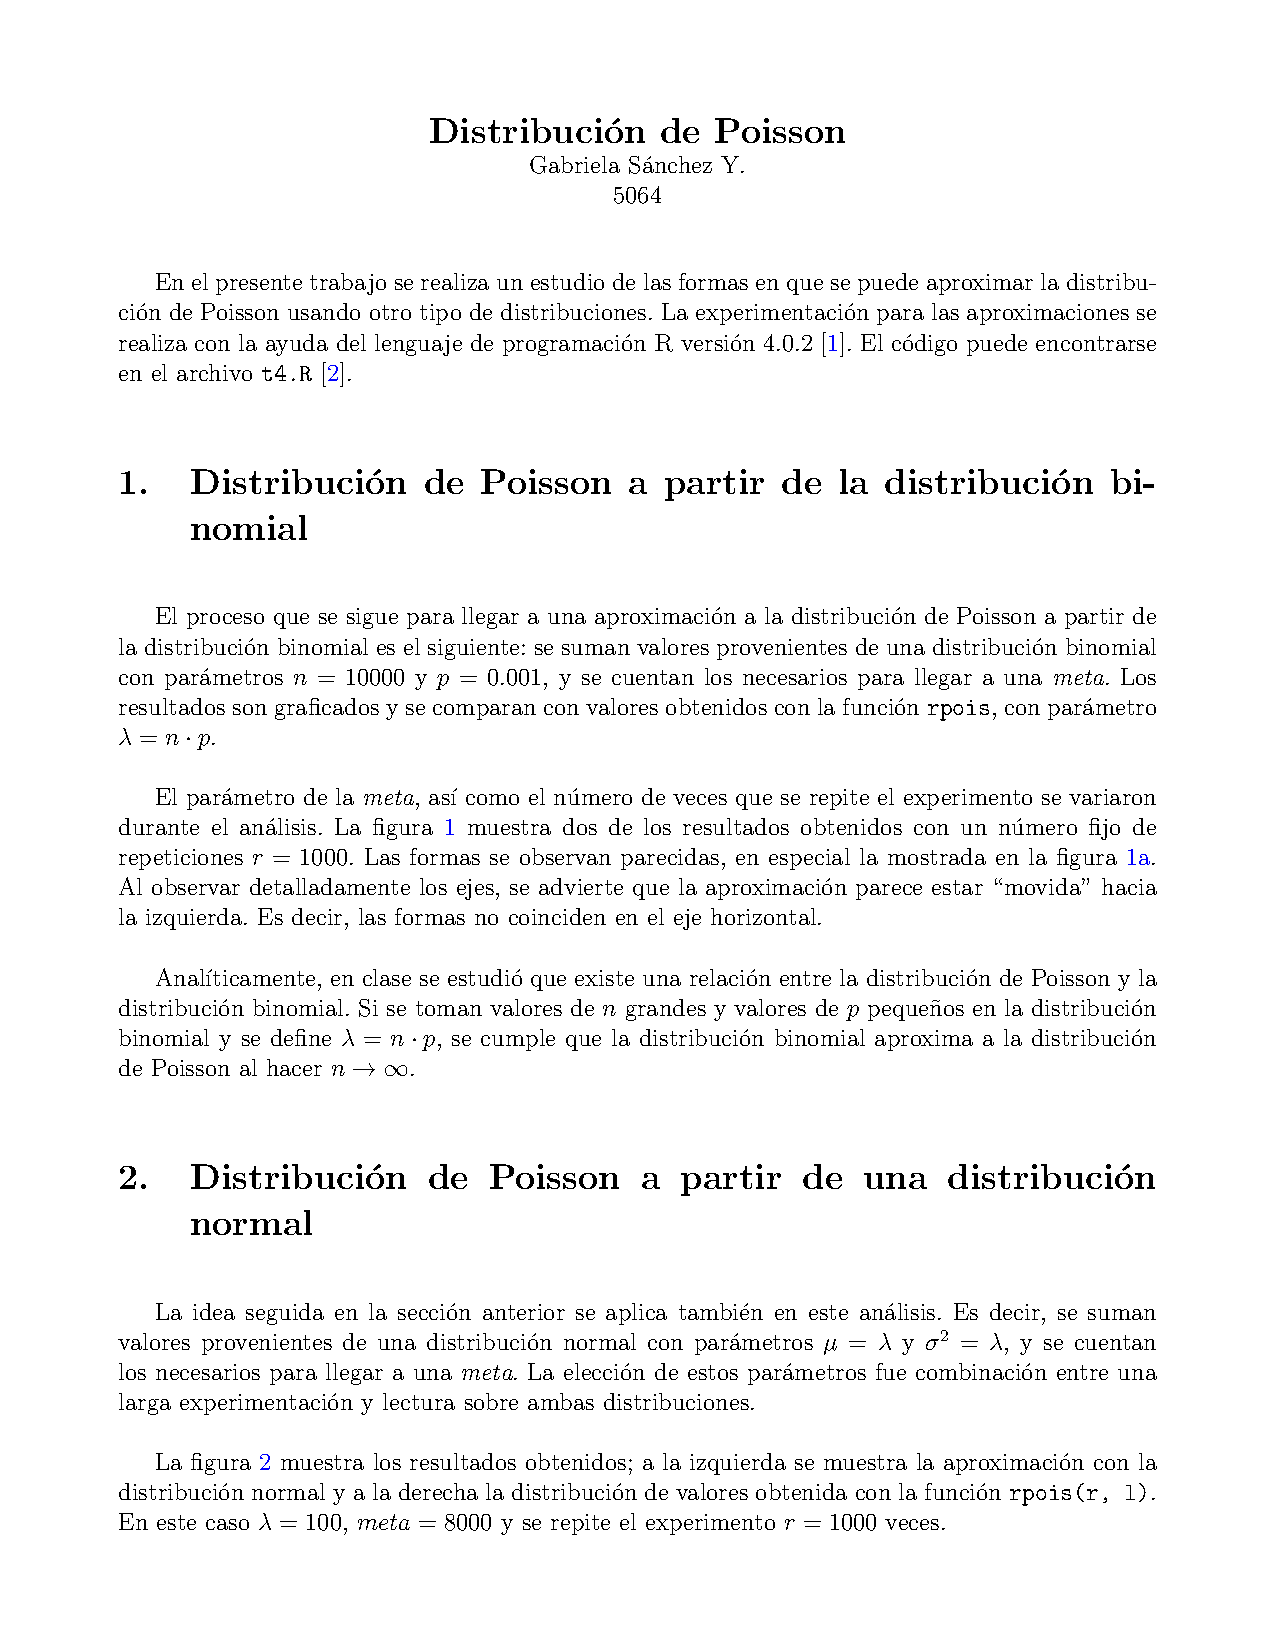
\includepdf[pages=-, addtotoc={1,chapter,4,{Tarea 4: Distribución de Poisson}, t4}]{t4.pdf}
	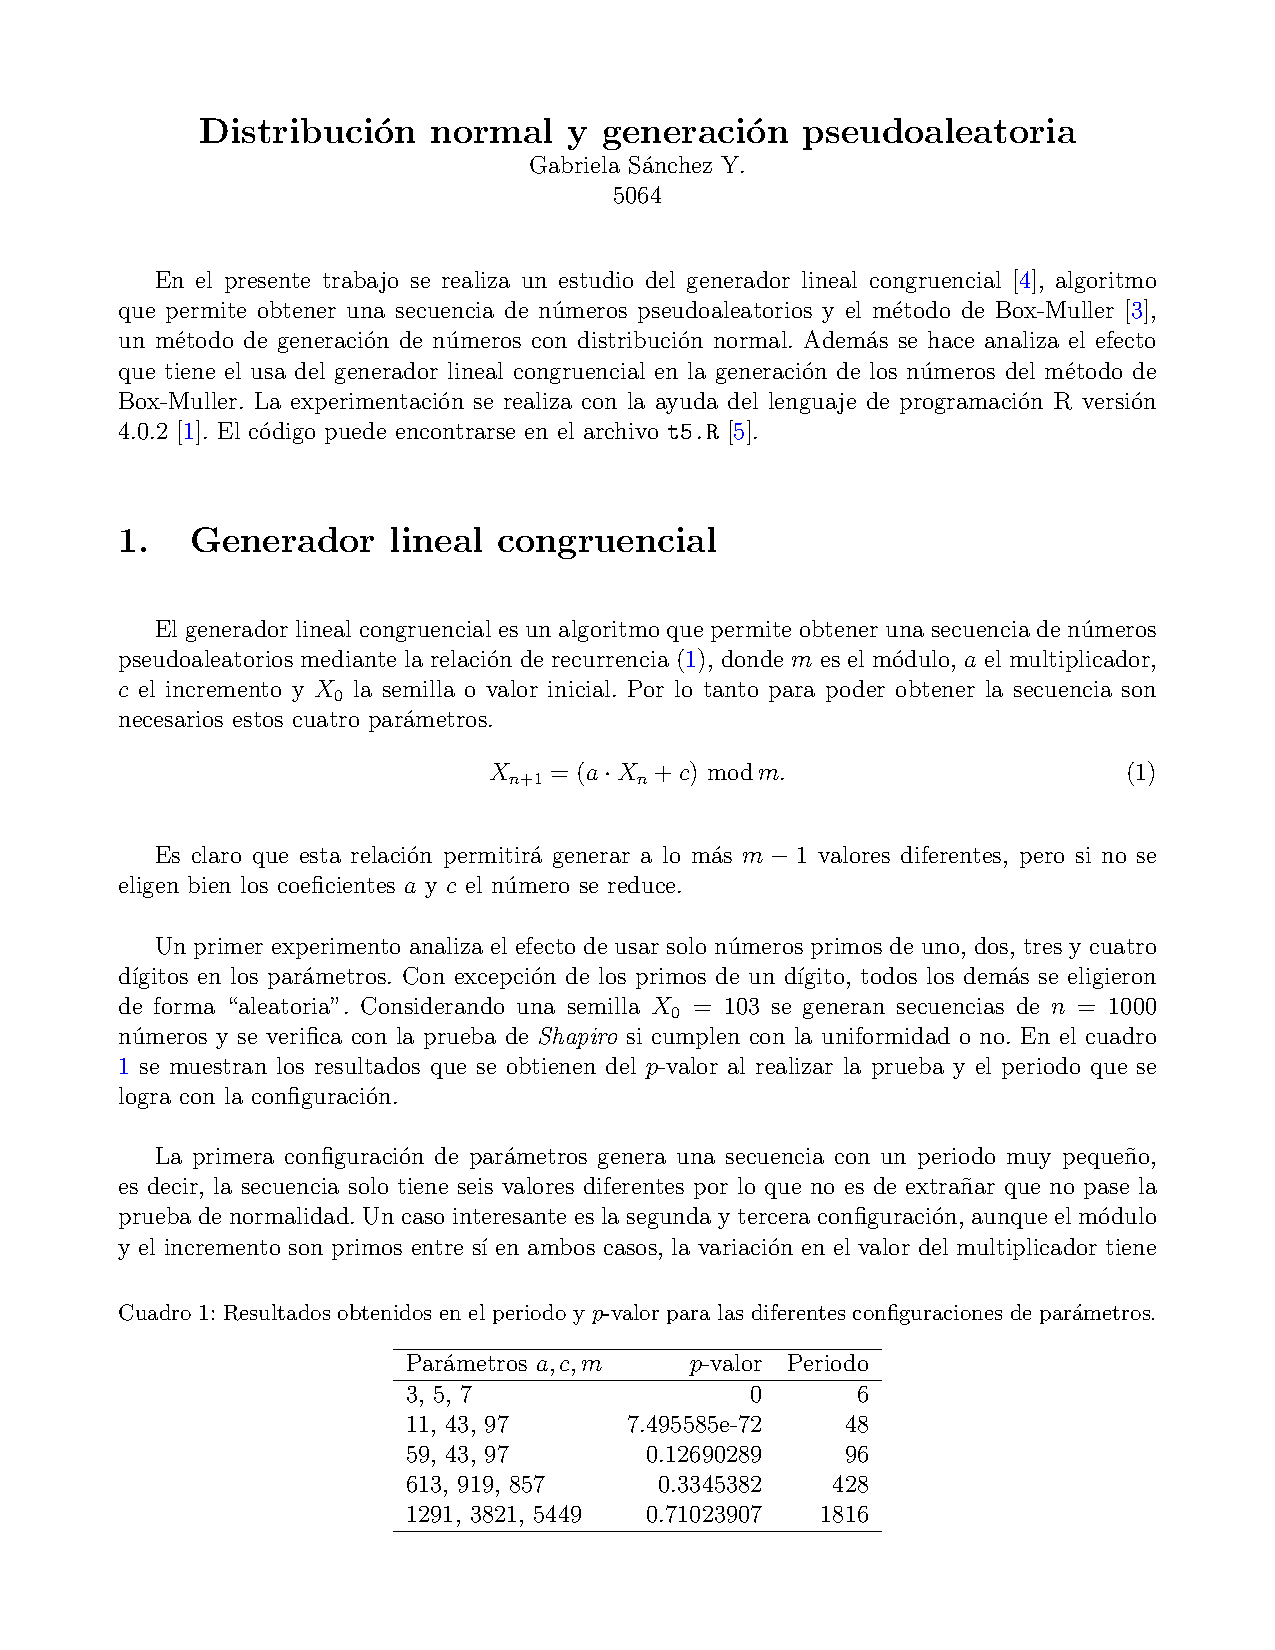
\includepdf[pages=-, addtotoc={1,chapter,5,{Tarea 5: Distribución normal y generación pseudoaleatoria}, t5}]{t5.pdf}
	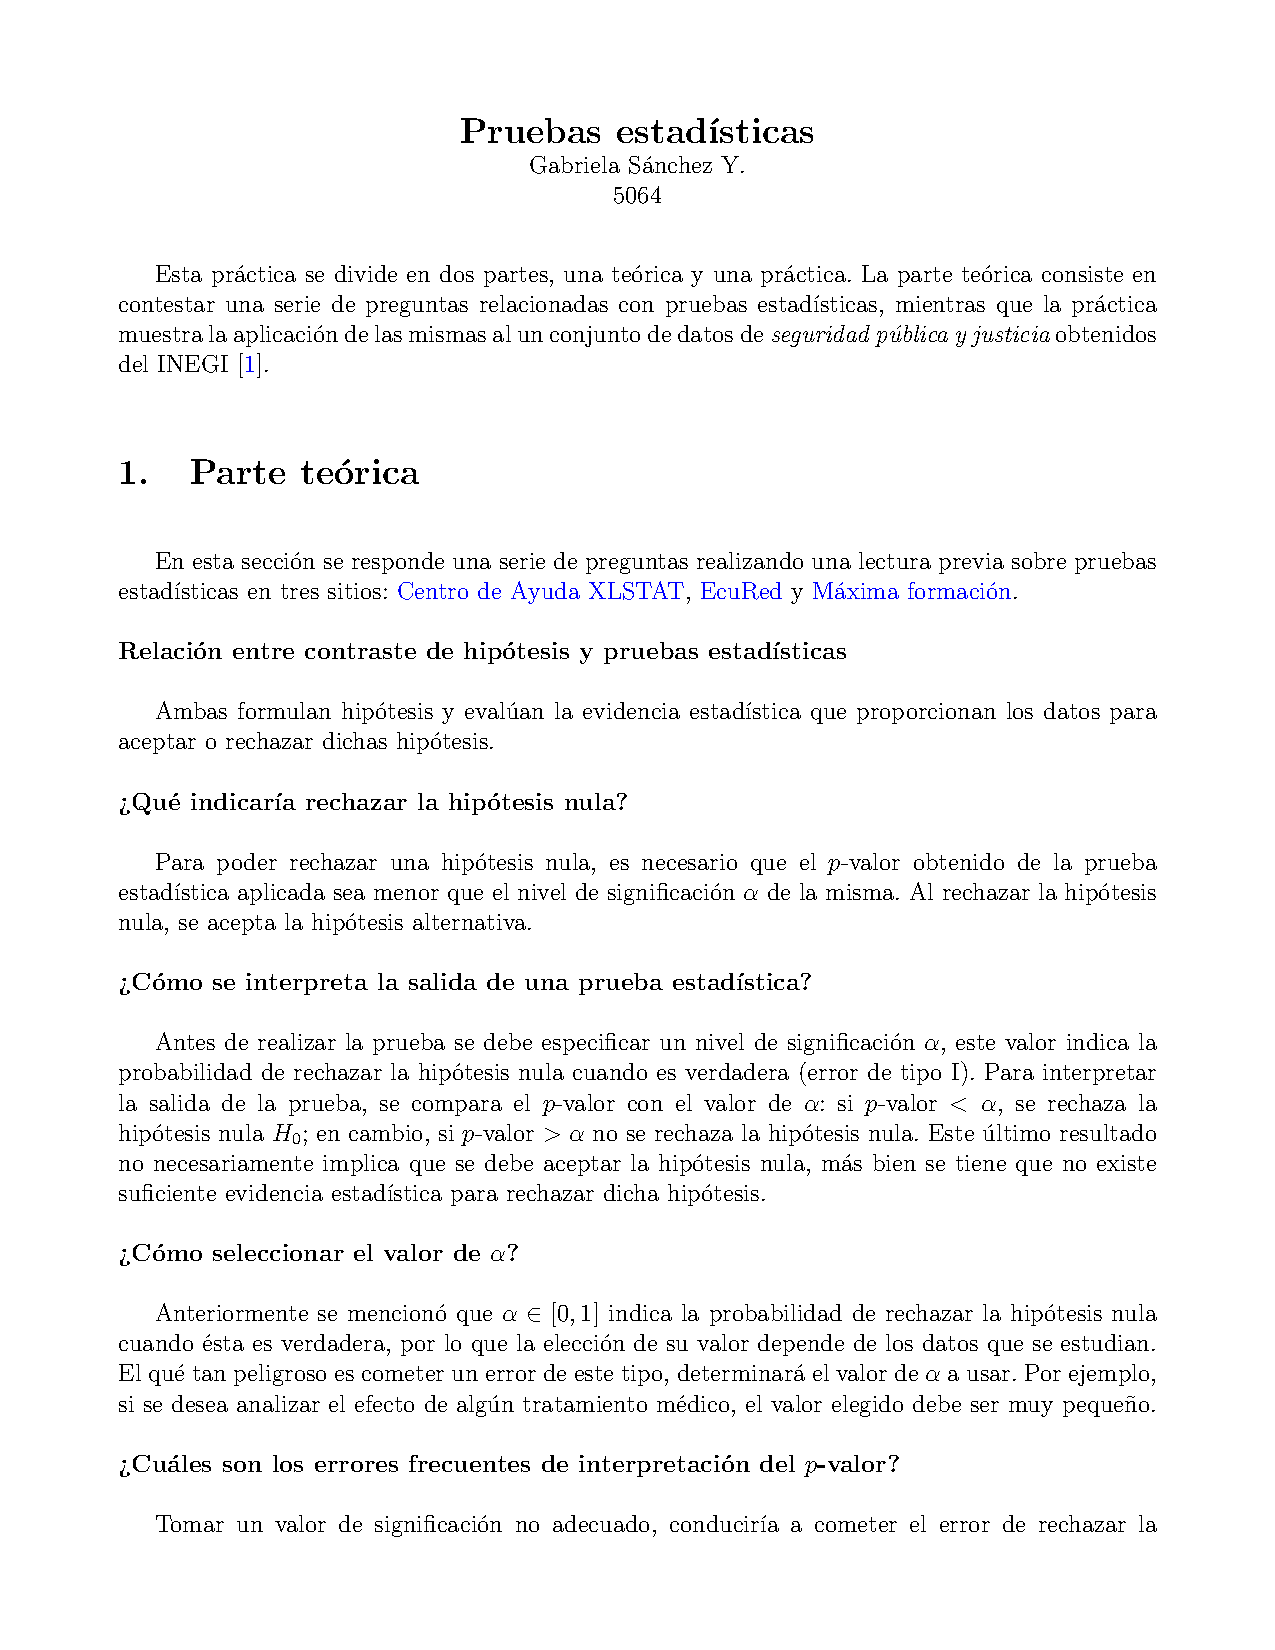
\includepdf[pages=-, addtotoc={1,chapter,6,{Tarea 6: Pruebas estadísticas}, t6}]{t6.pdf}
	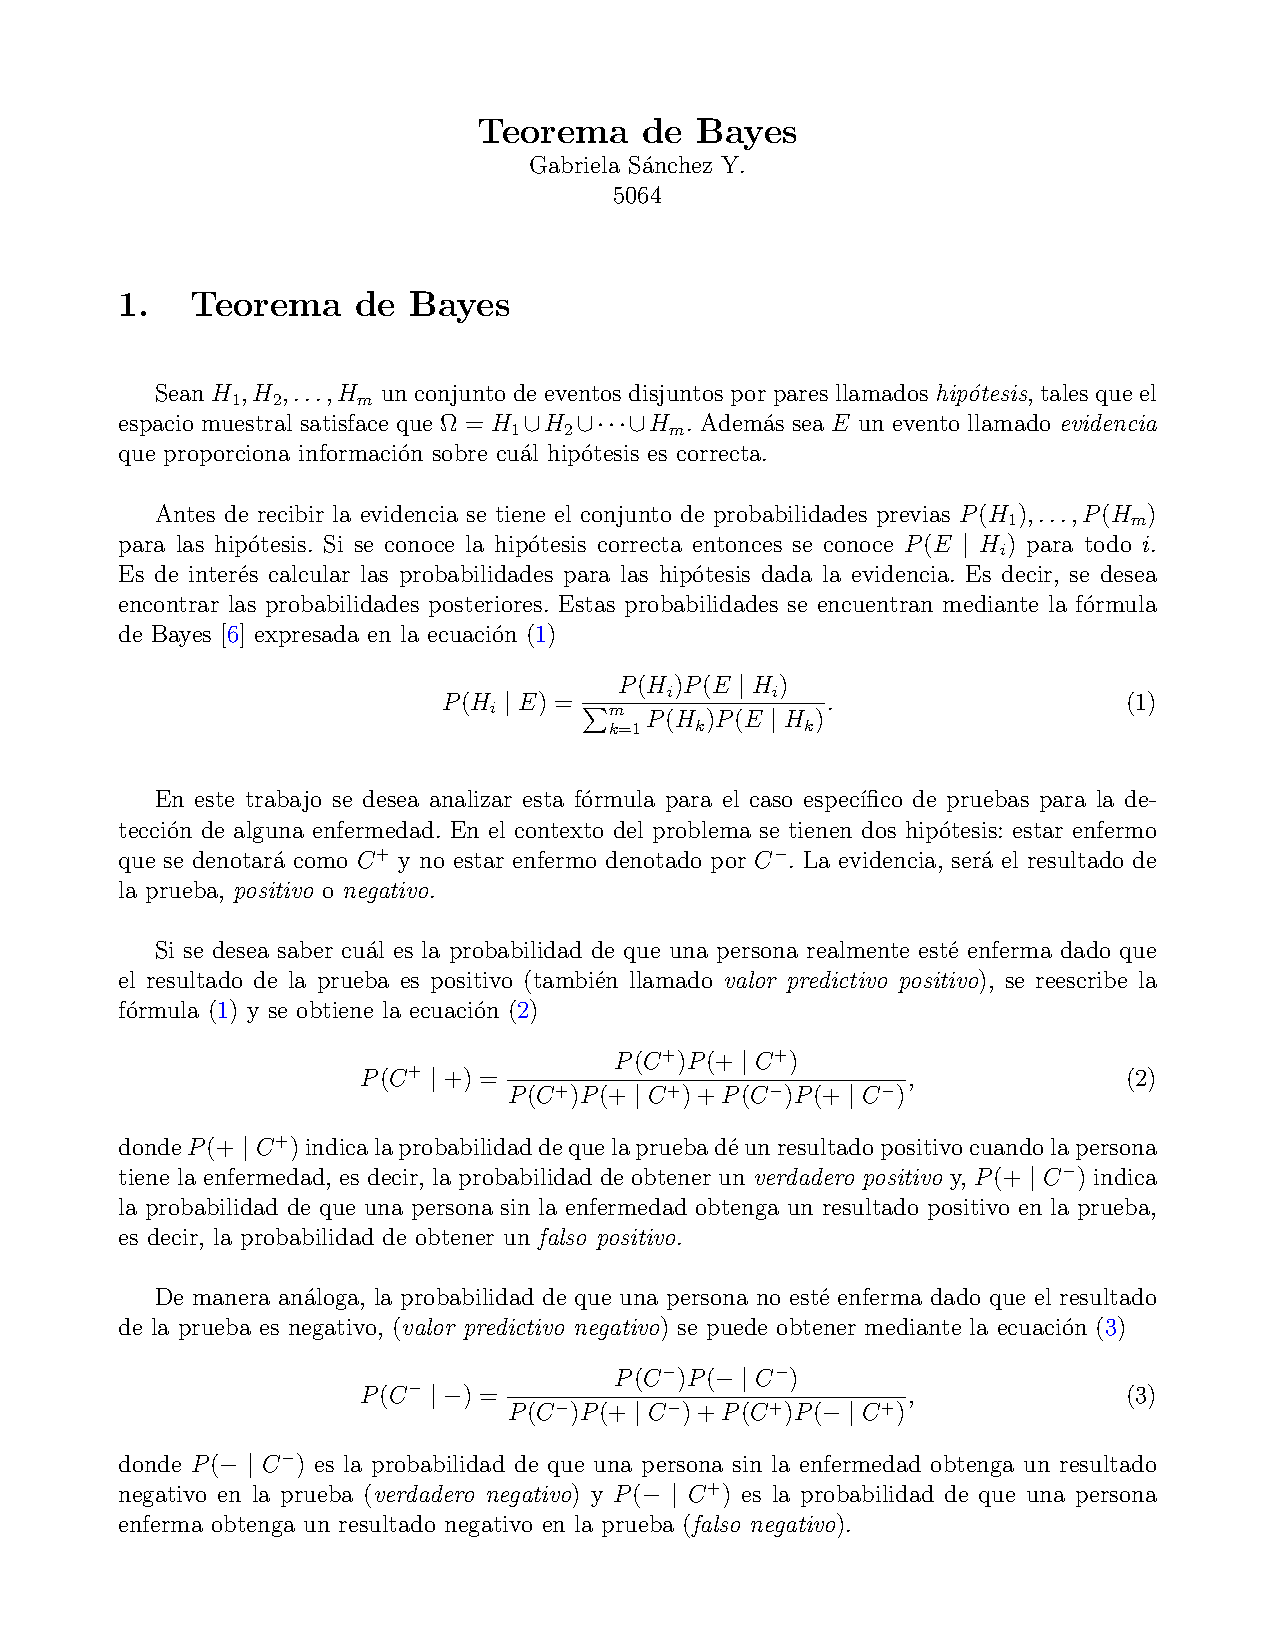
\includepdf[pages=-, addtotoc={1,chapter,7,{Tarea 8: Teorema de Bayes}, t8}]{t8.pdf}
	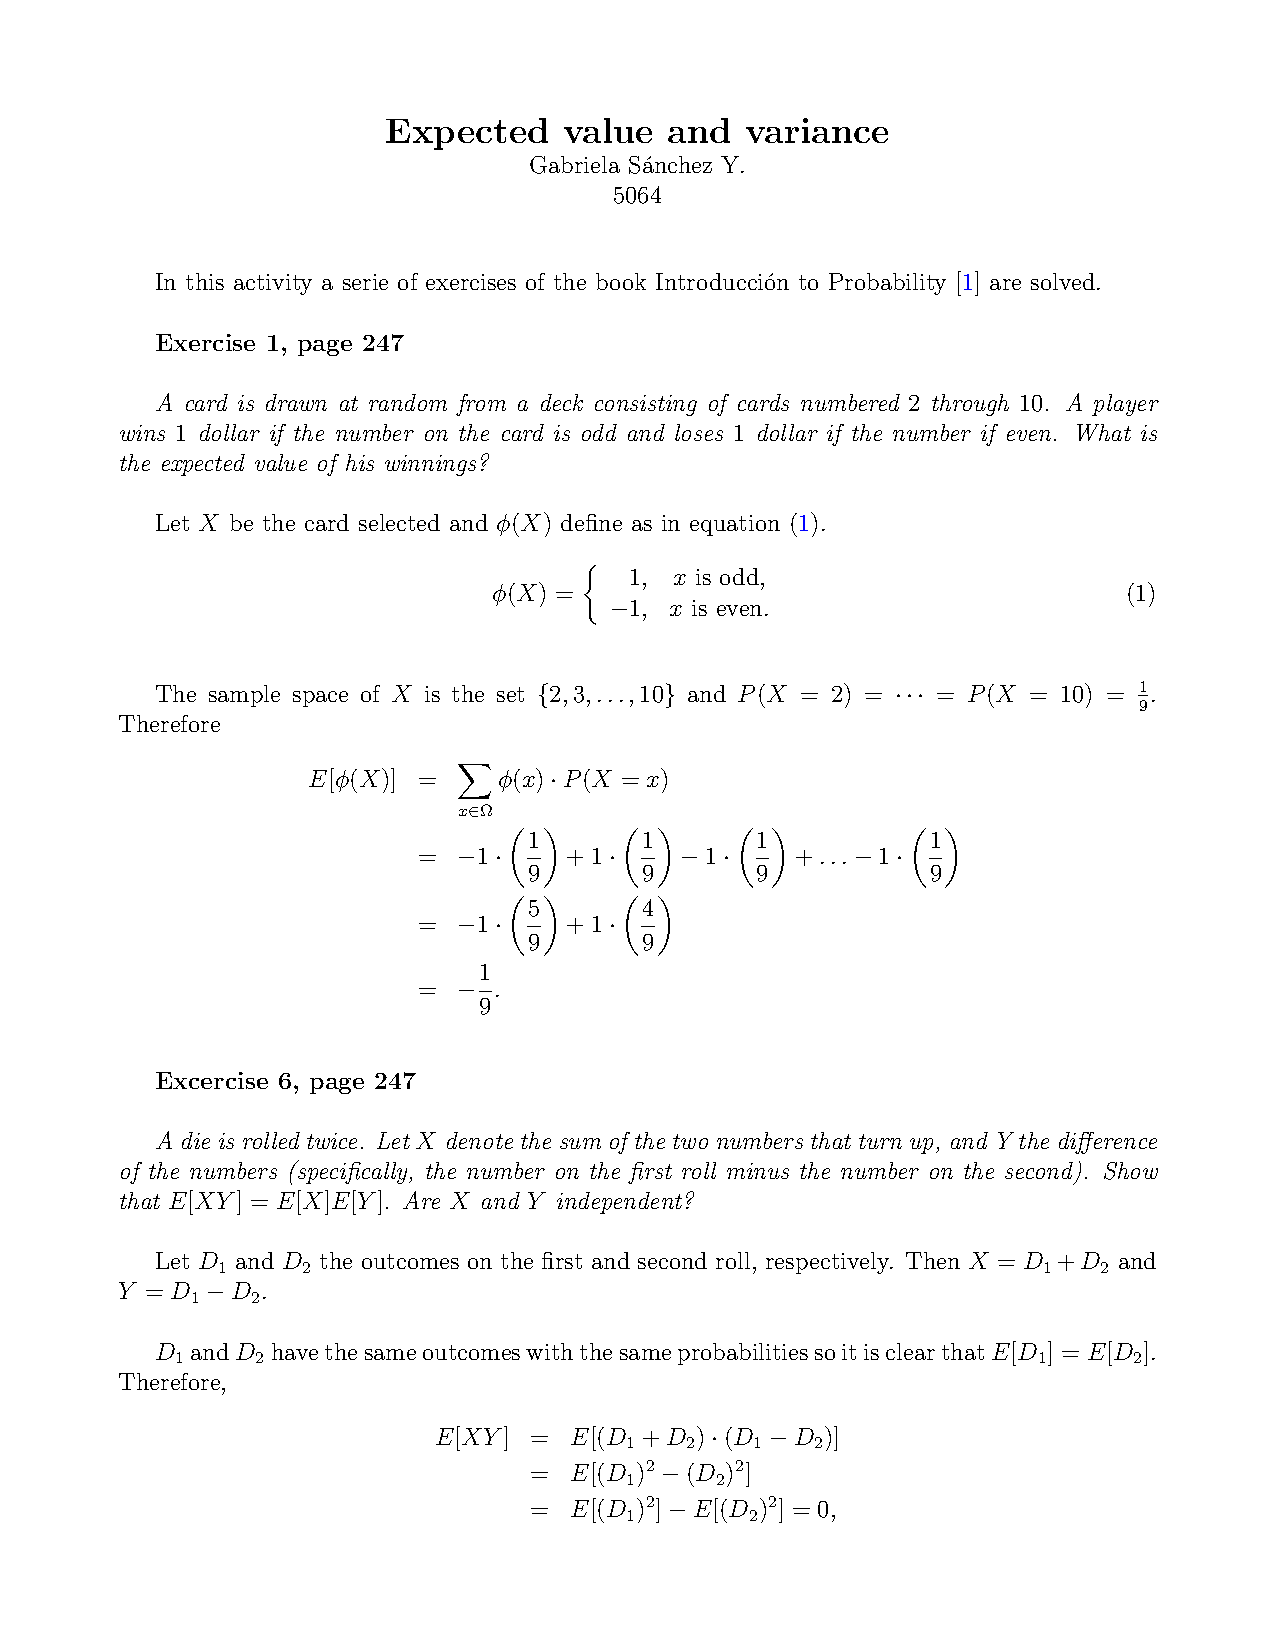
\includepdf[pages=-, addtotoc={1,chapter,8,{Tarea 9: Valor esperado y varianza}, t9}]{t9.pdf}
	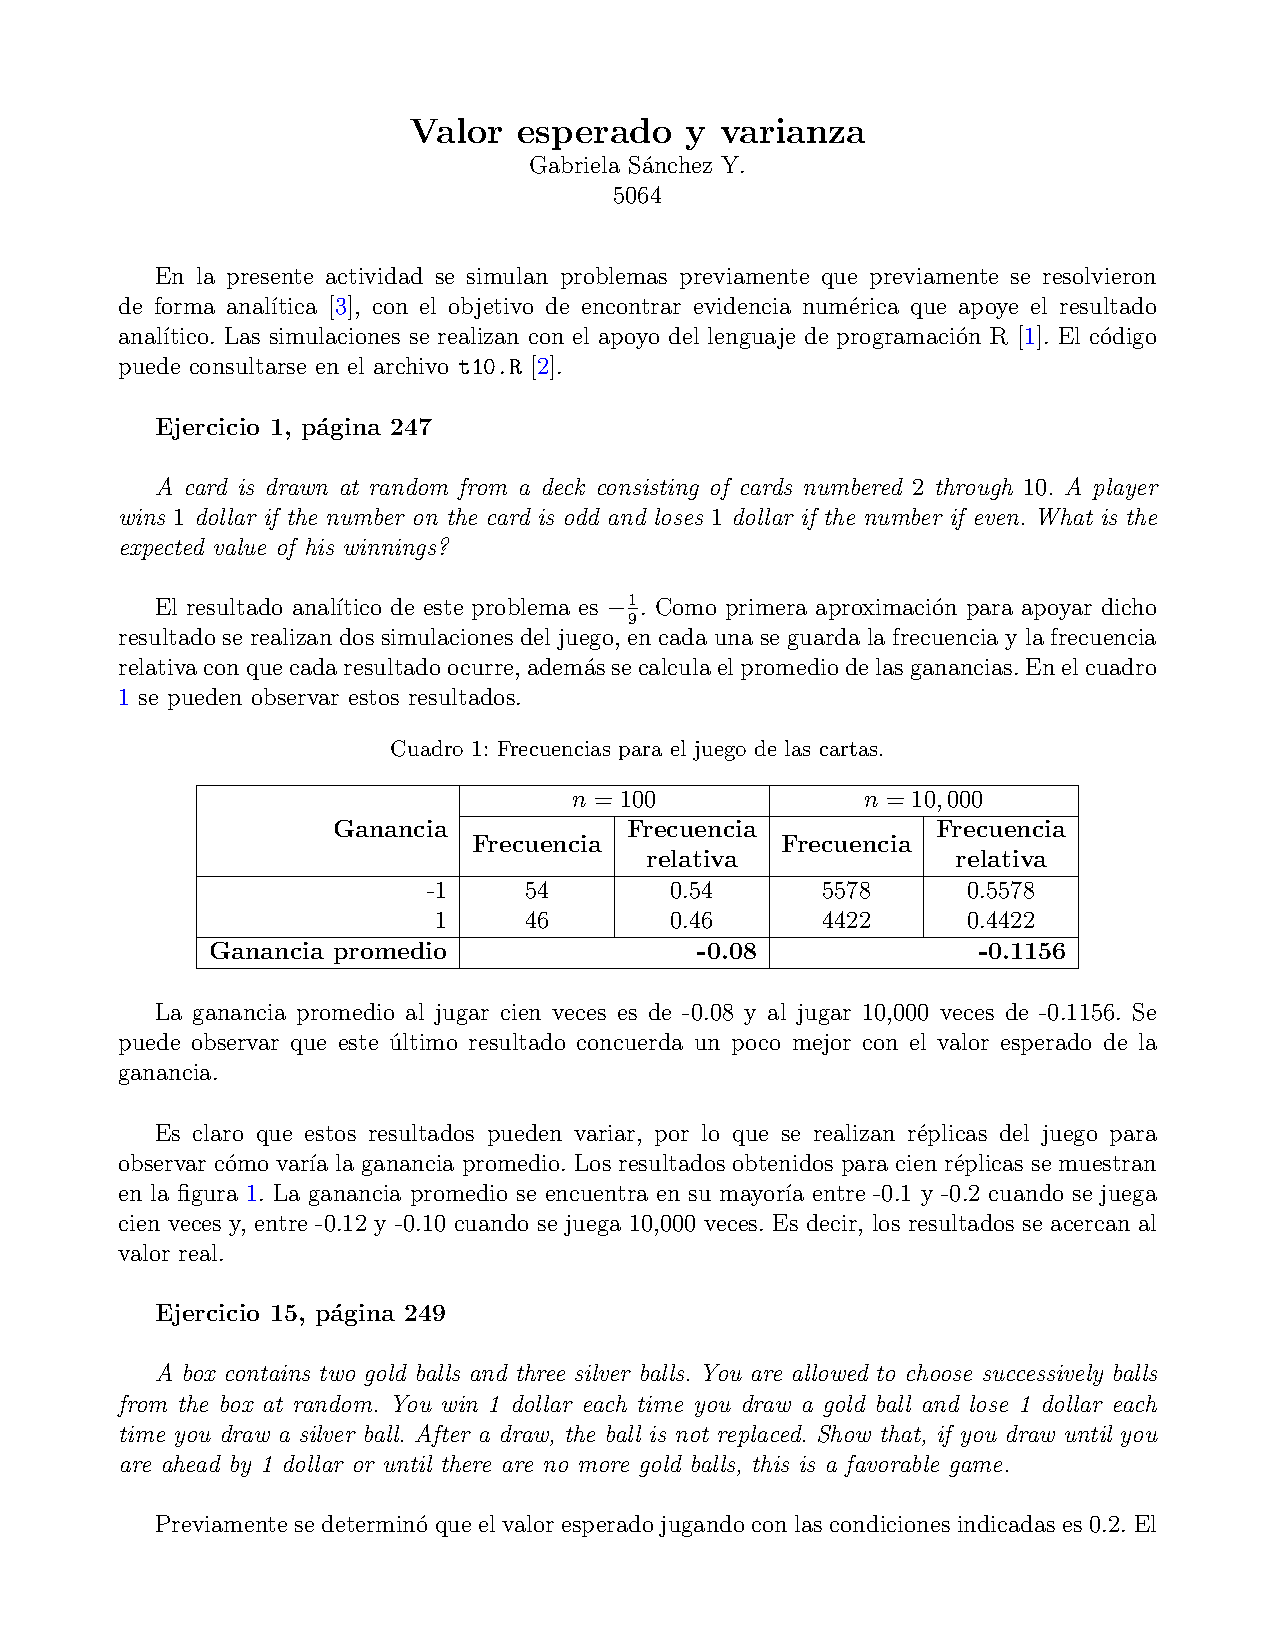
\includepdf[pages=-, addtotoc={1,chapter,9,{Tarea 10: Valor esperado y varianza (parte experimental)}, t10}]{t10.pdf}
	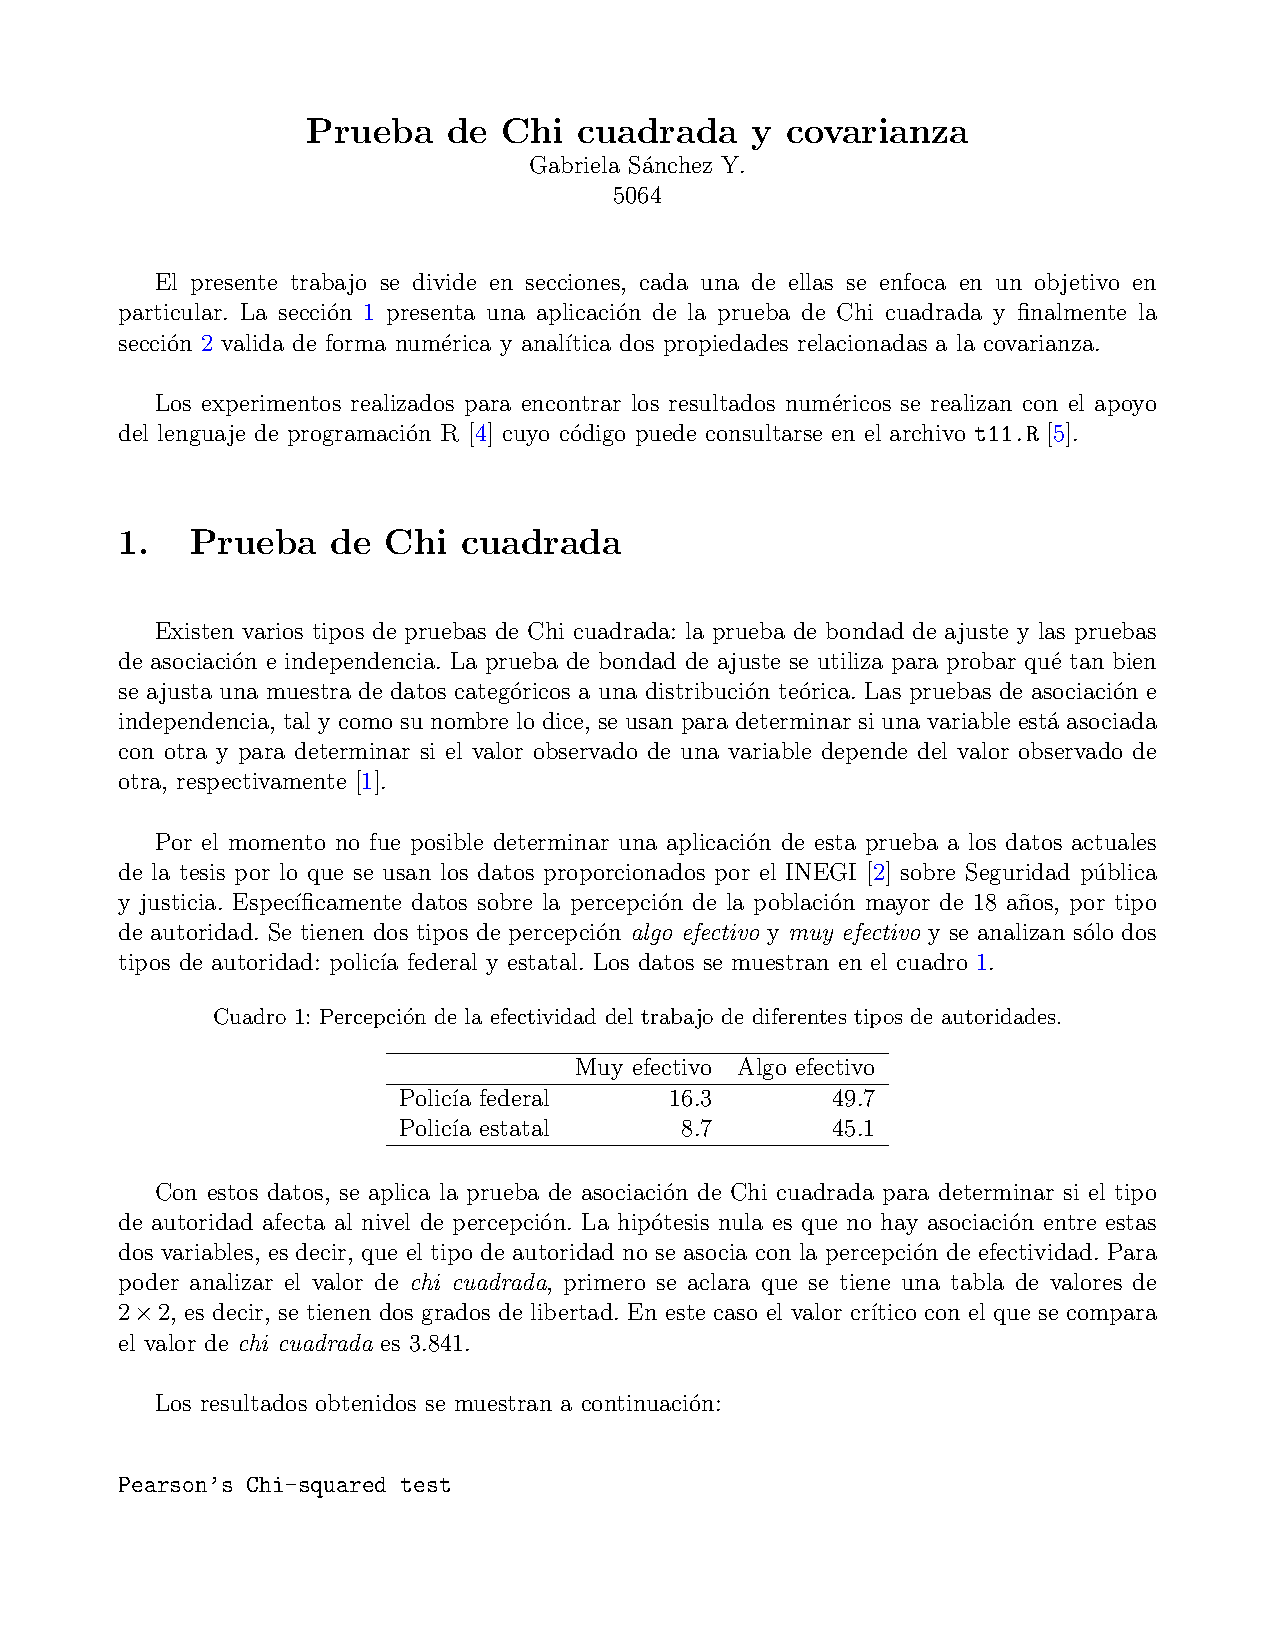
\includepdf[pages=-, addtotoc={1,chapter,10,{Tarea 11: Prueba de Chi cuadrada y covarianza}, t11}]{t11.pdf}
	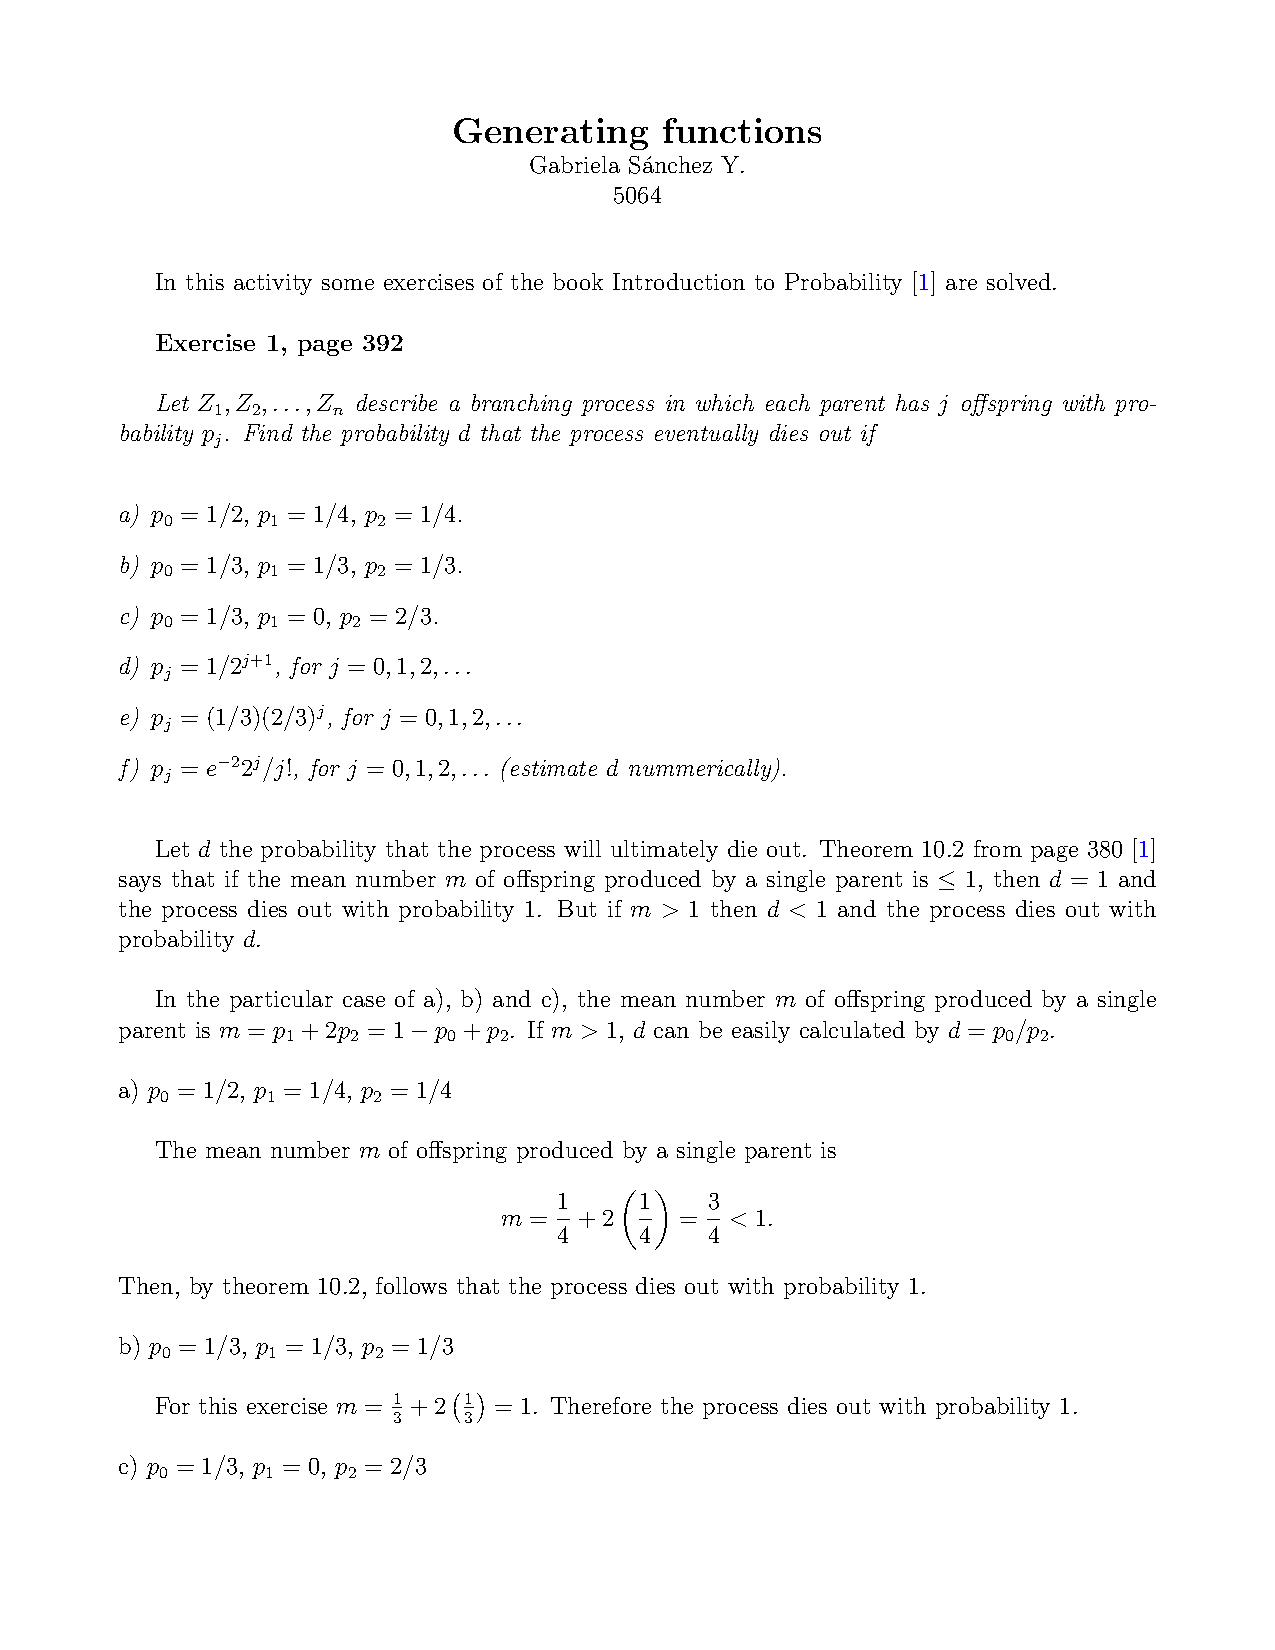
\includepdf[pages=-, addtotoc={1,chapter,11,{Tarea 12: Funciones generadoras}, t12}]{t12.pdf}
	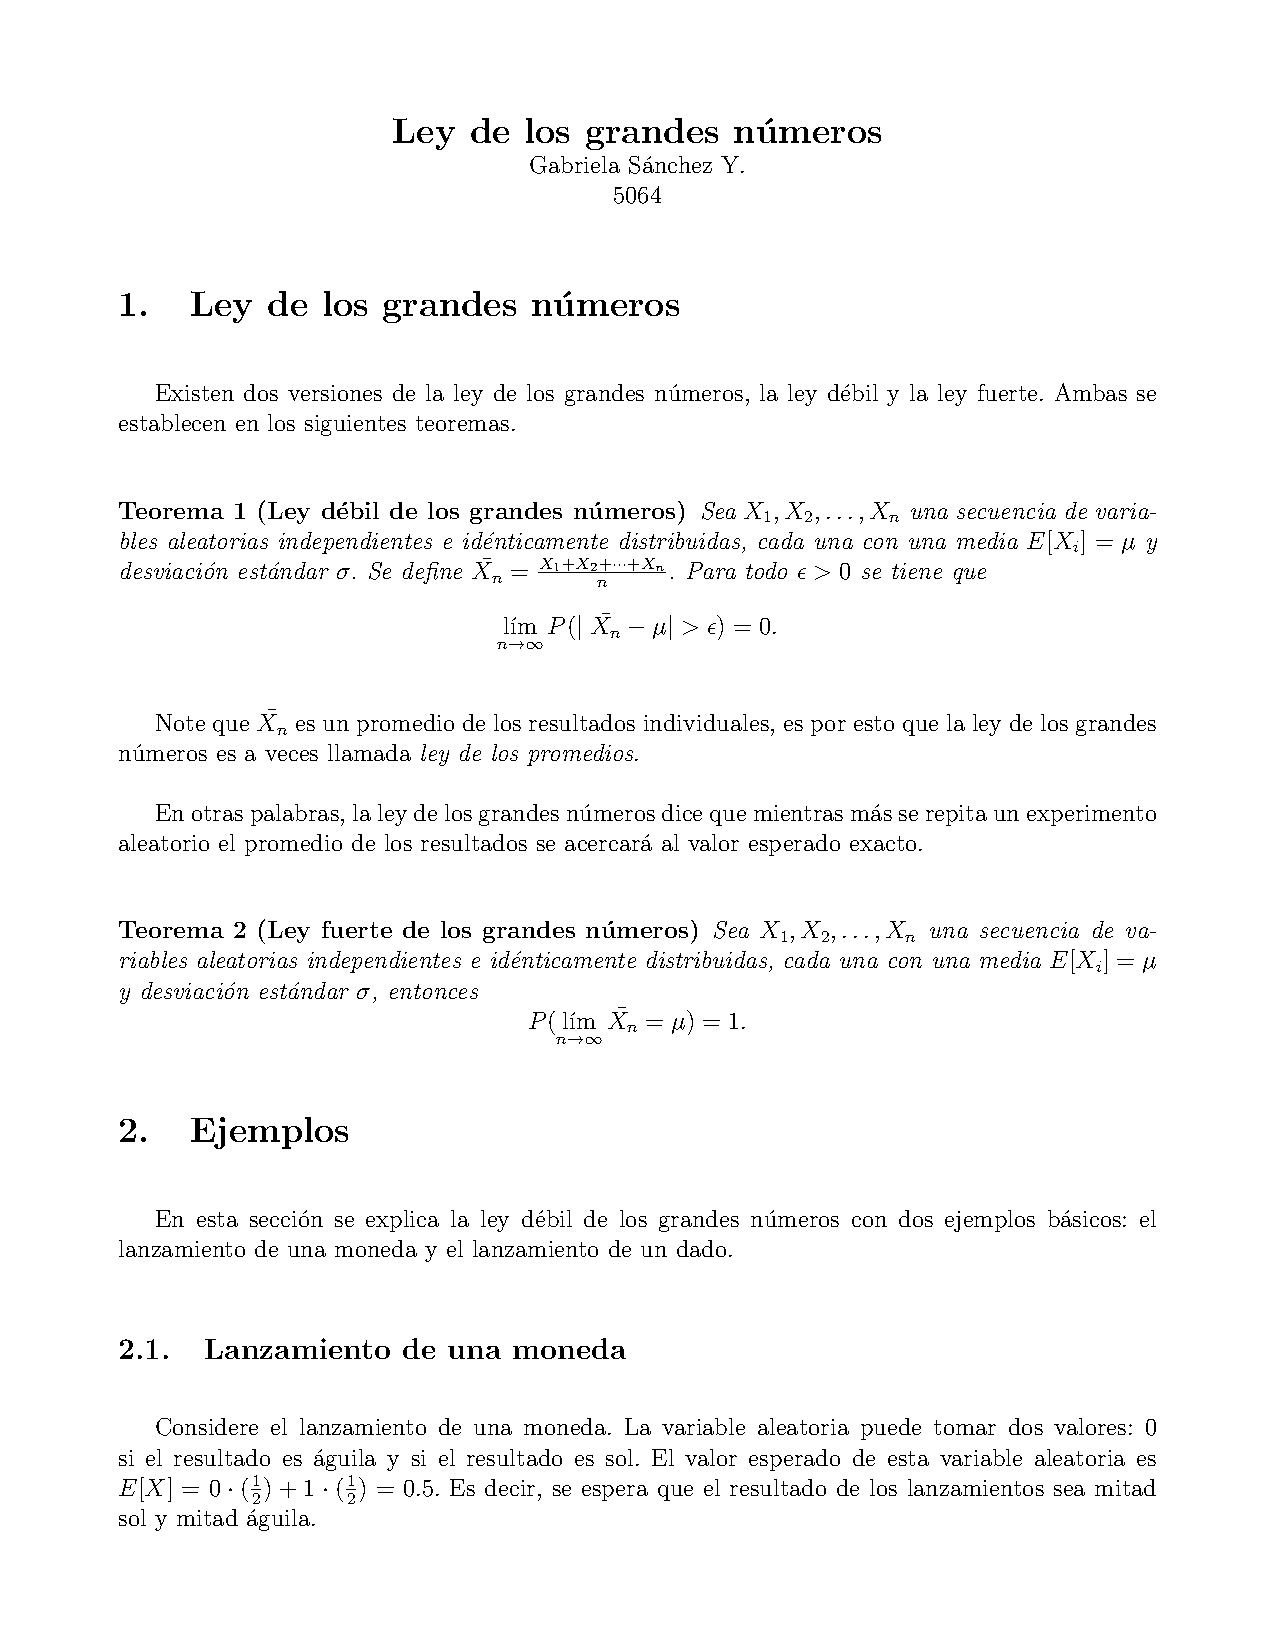
\includepdf[pages=-, addtotoc={1,chapter,12,{Tarea 13: Ley de los grandes números}, t13}]{t13.pdf}
	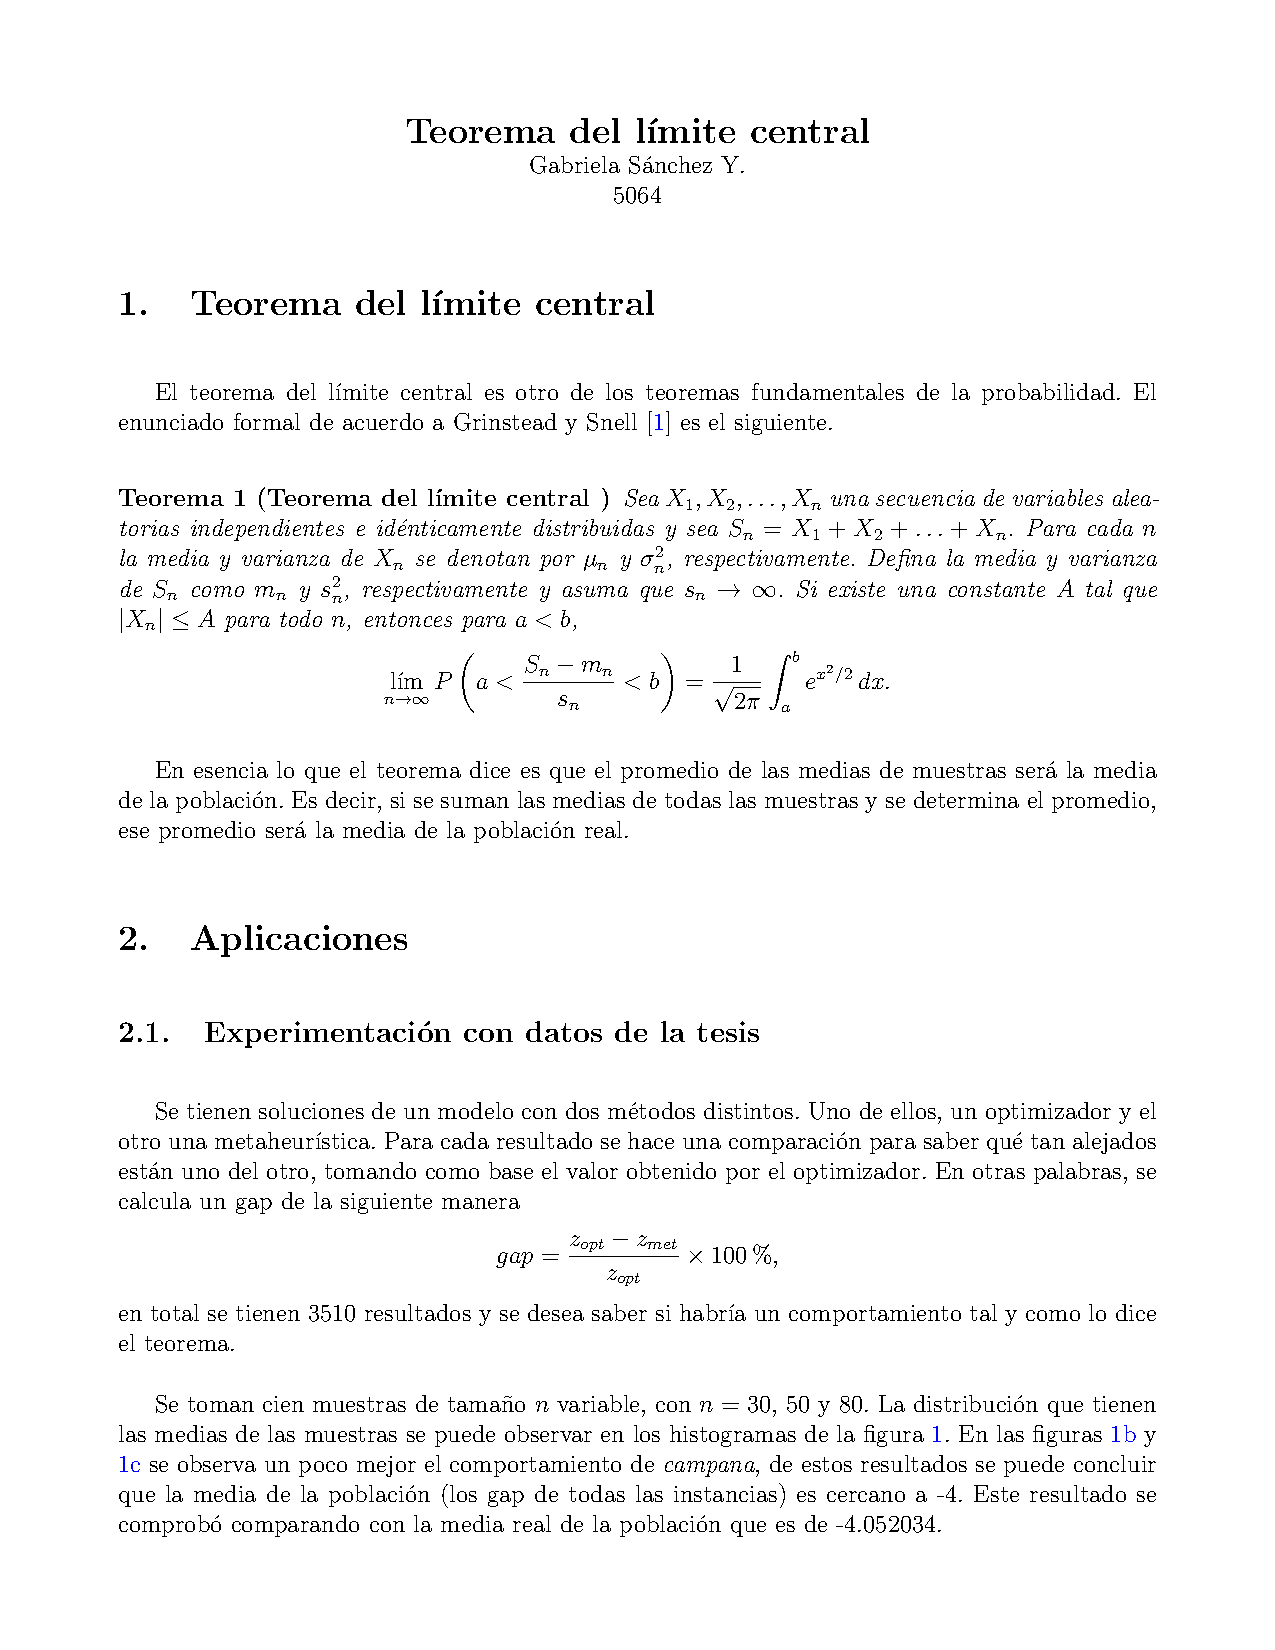
\includepdf[pages=-, addtotoc={1,chapter,13,{Tarea 14: Teorema del límite central}, t14}]{t14.pdf}
	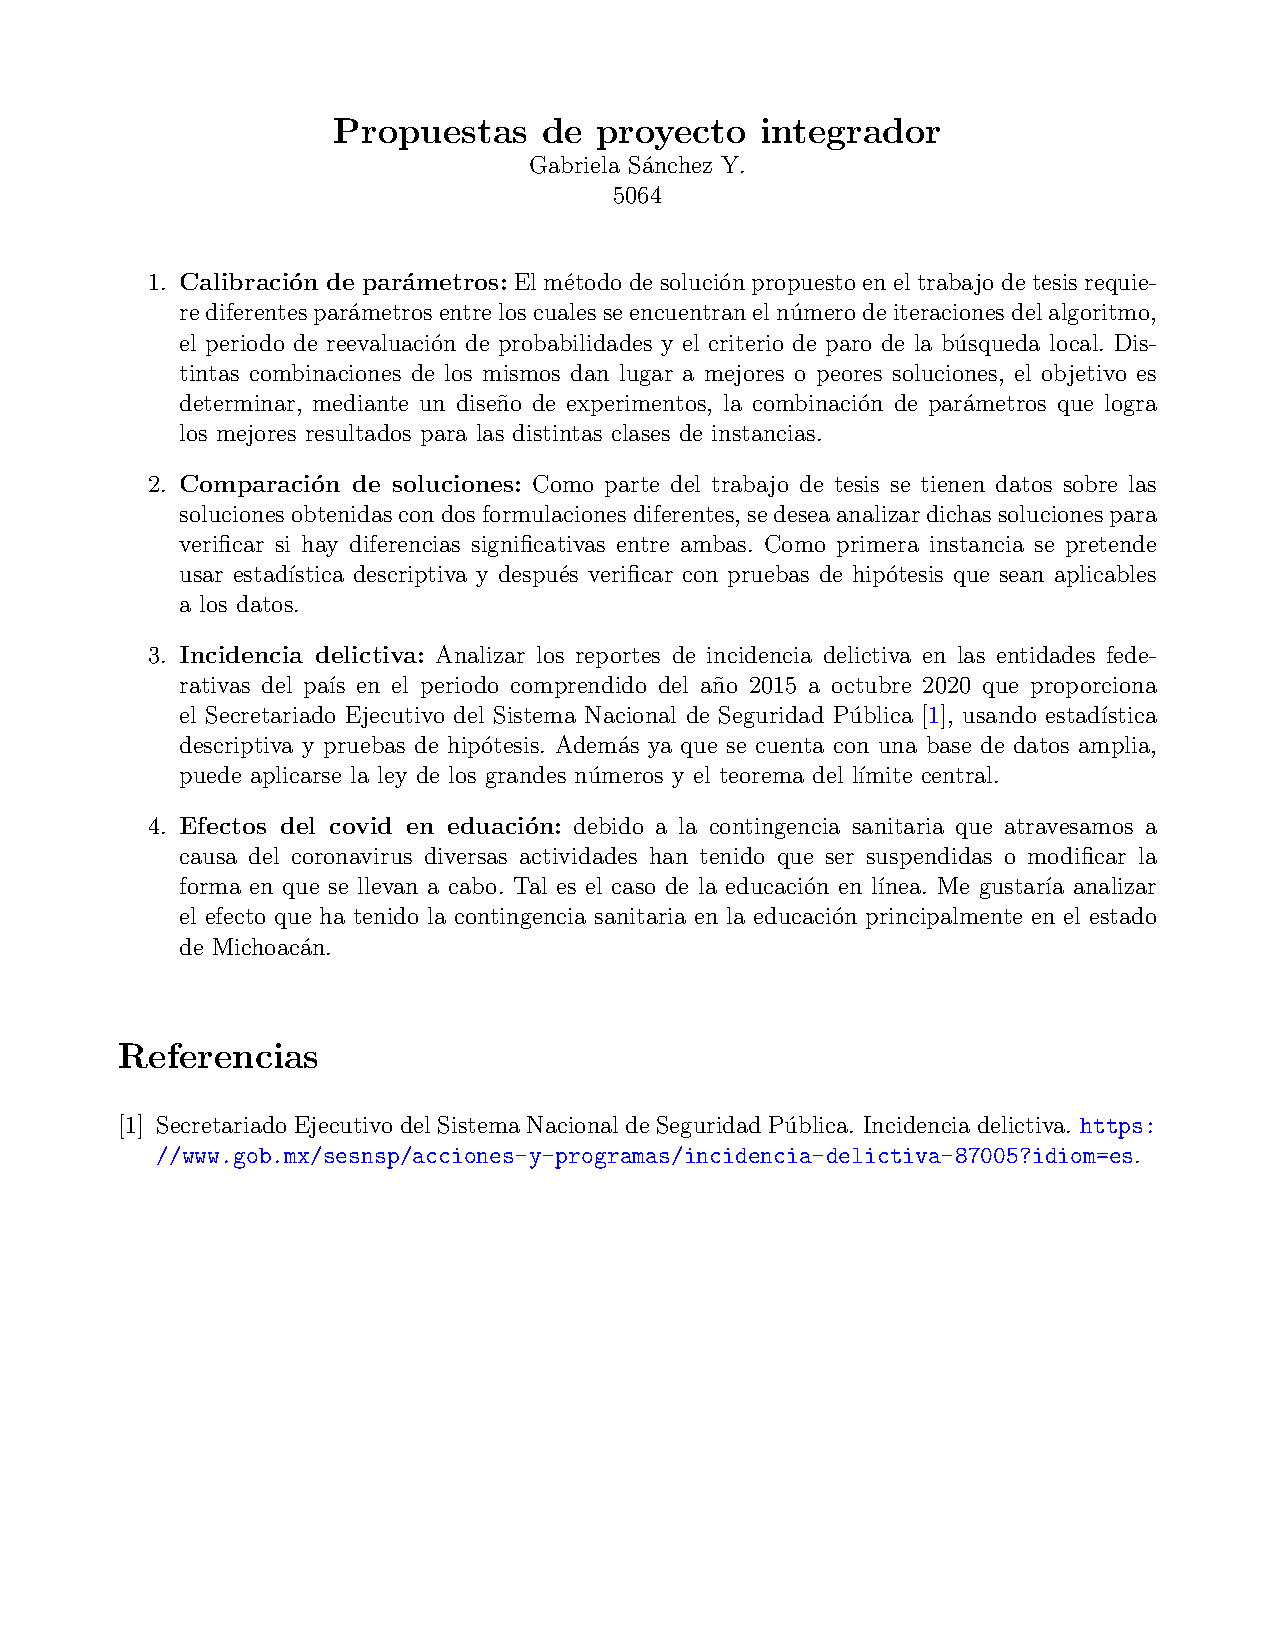
\includepdf[pages=-, addtotoc={1,chapter,14,{Tarea 15: Propuestas de proyecto integrador}, t15}]{t15.pdf}
	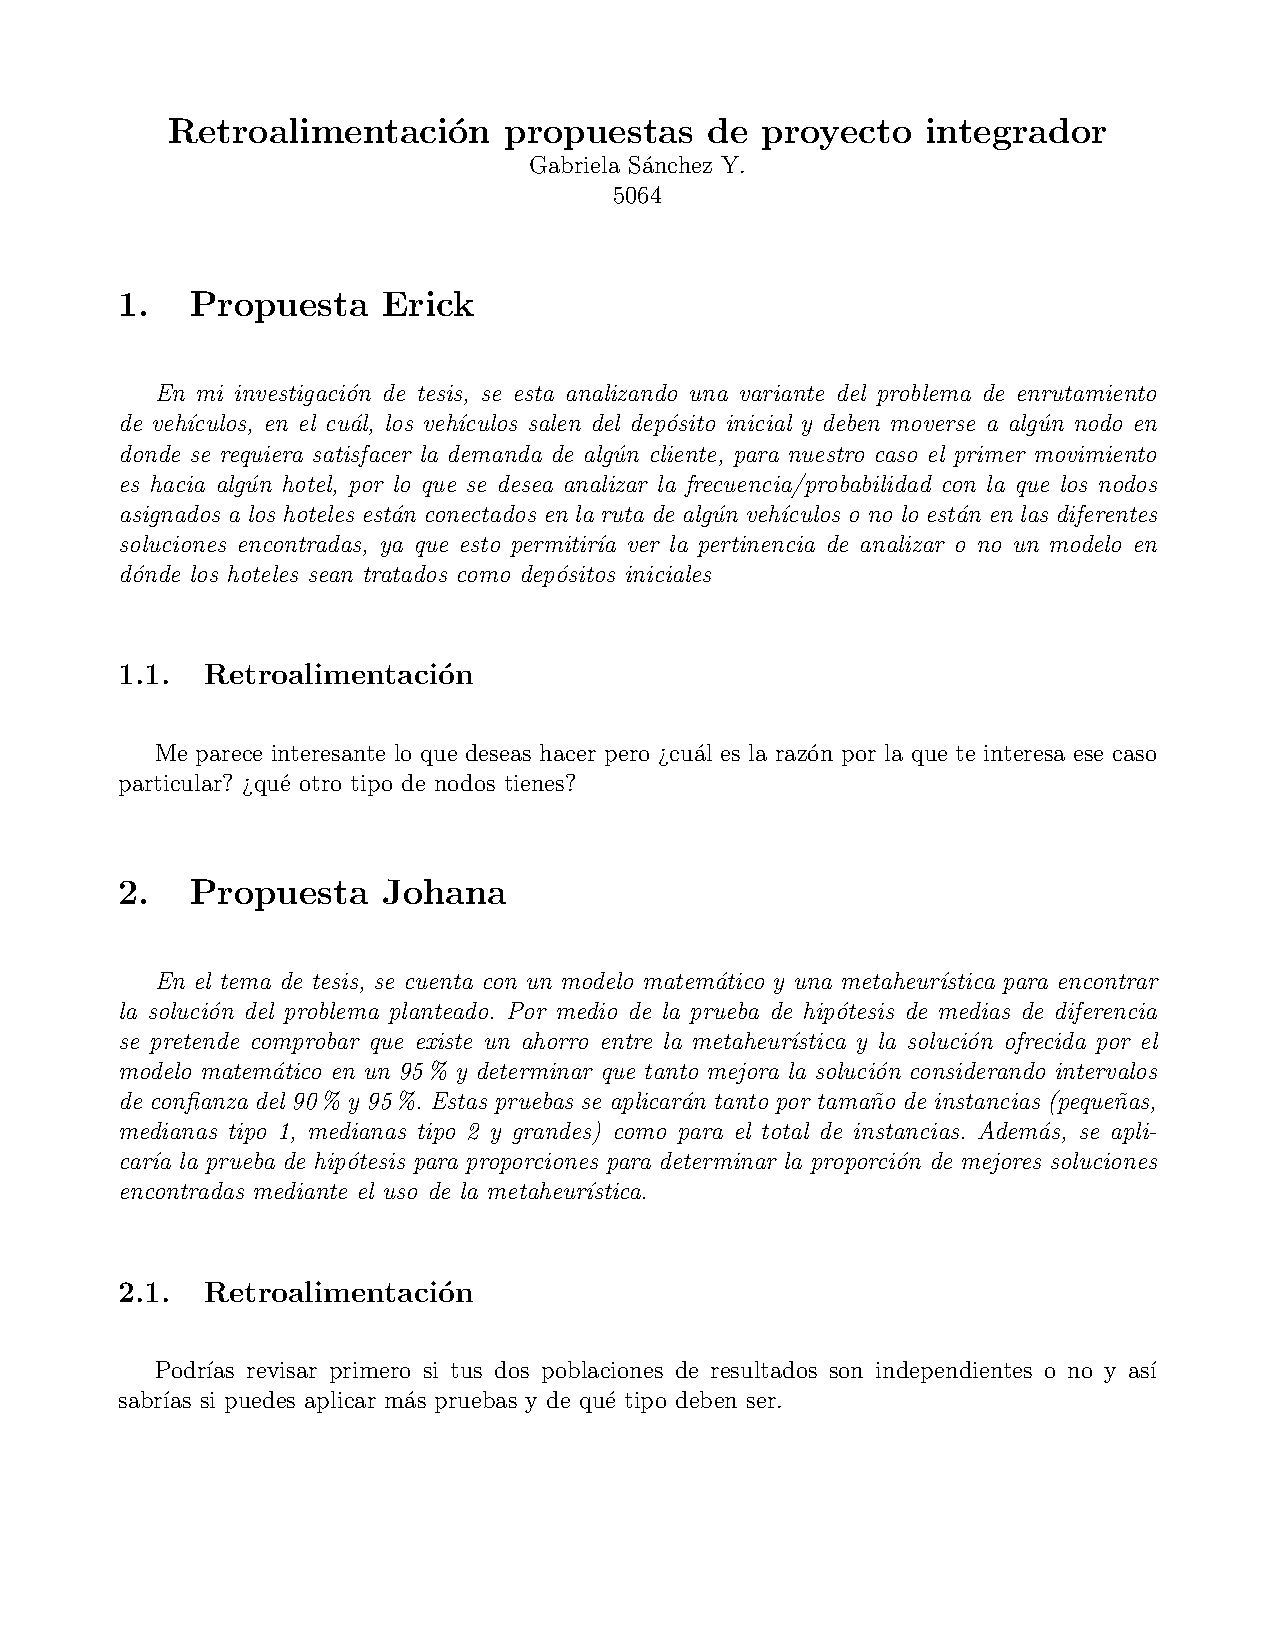
\includepdf[pages=-, addtotoc={1,chapter,15,{Tarea 16: Retroalimentación propuestas de proyecto integrador}, t16}]{t16.pdf}
	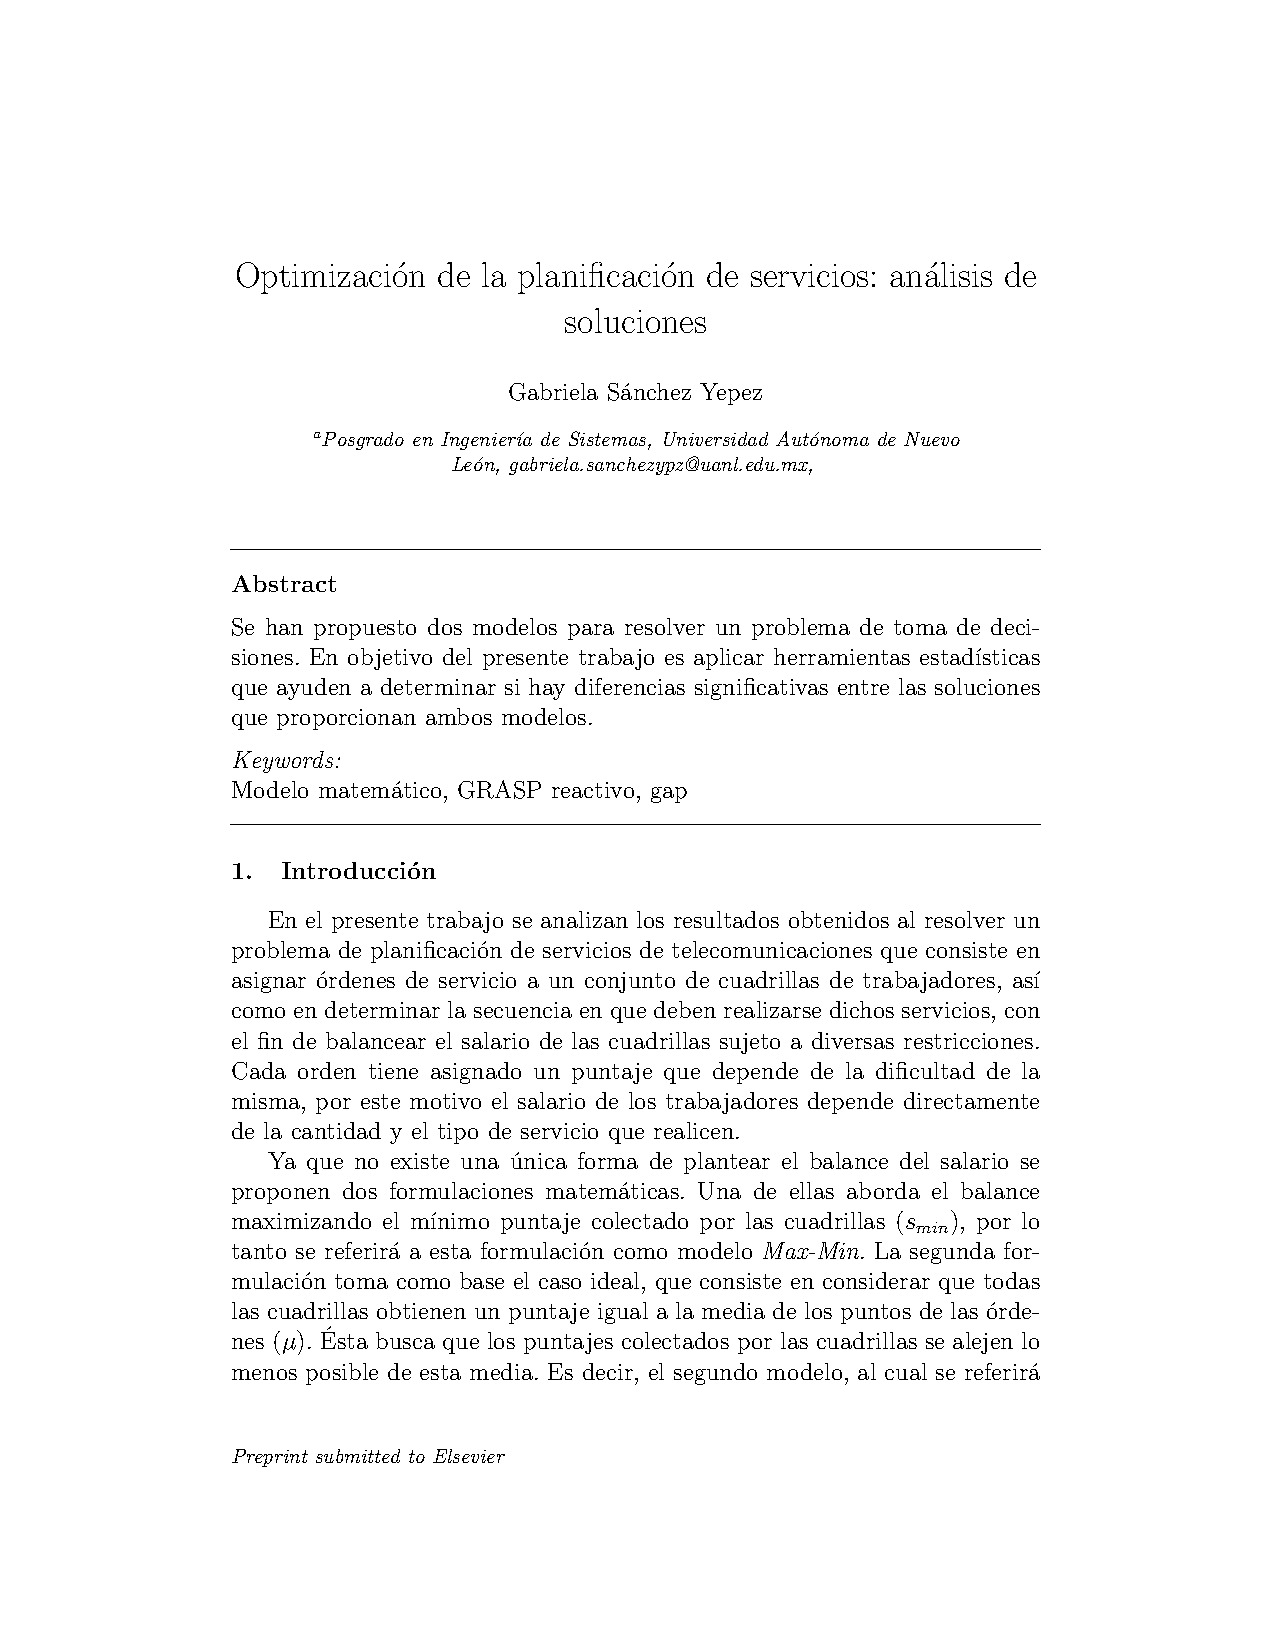
\includepdf[pages=-, addtotoc={1,chapter,16,{Proyecto integrador}, proyecto}]{proyecto.pdf}
	%\includepdf[pages=-,addtotoc={4,chapter,1,{A Great Chapter},greatchap}]{trial.pdf}
\end{document}
